%\documentclass[first,firstsupp,handout,compress,notes,navigation]{ETHclass} 
%\documentclass[first,firstsupp,handout,lastsupp]{ETHclass} 
\documentclass[first,firstsupp,lastsupp,handout,last,hyperref,table]{ETHclass} 
%\documentclass[first,firstsupp]{ETHclass}
\usepackage{etex}

\usepackage{adjustbox}
\usepackage{amsmath}
\usepackage{amssymb}
\usepackage{animate}
\usepackage{booktabs}
\usepackage{charter}
\usepackage{enumitem}
\usepackage{etoolbox}
\usepackage{ifthen}
\usepackage{longtable}
\usepackage{mathrsfs}
\usepackage{multicol}
\usepackage{pgf}
\usepackage{pgfplots}
\usepackage{pifont}
\usepackage{ragged2e}
\usepackage{standalone}
\usepackage[caption=false]{subfig}
\usepackage{tabularx}
\usepackage{tikz}
\usepackage{verbatim}
\usepackage{xcolor}
\usepackage{hyperref}

\pgfplotsset{compat=1.7}

\setbeamertemplate{navigation symbols}{}
\usetikzlibrary{arrows,decorations.pathreplacing,positioning,shapes,shadows}

%\usepackage[style=numeric-comp]{biblatex}

%\usepackage{lipsum}

%\usetikzlibrary{fit}
\usetikzlibrary{arrows}
\usetikzlibrary{trees}

% Options for beamer:
%
% 9,10,11,12,13,14,17pt  Fontsizes
% 
% compress: navigation bar becomes smaller
% t       : place contents of frames on top (alternative: b,c)
% handout : handoutversion
% notes   : show notes
% notes=onlyslideswithnotes
%
%hyperref={bookmarksopen,bookmarksnumbered} : Needed for menues in
%                                             acrobat. Also need
%                                             pdftex as option or 
%                                             compile with
% pdflatex '\PassOptionsToPackage{pdftex,bookmarksopen,bookmarksnumbered}{hyperref} \input{file}'

%\usepackage{beamerseminar}
%\usepackage[accumulated]{beamerseminar}
                                % remove ``accumulated'' option
                                % for original behaviour
%\usepackage{beamerbasenotes}
%\setbeamertemplate{note page}[plain] 
%\setbeameroption{notes on second screen}

%\setbeamertemplate{note page}[plain] 
\setbeamertemplate{note page}{\ \\[.3cm]
\textbf{\color{blue}Notes:}\\%[0.1cm]
{\footnotesize %\tiny
\insertnote}}
%\setbeameroption{notes on second screen}


%\setbeamertemplate{navigation symbols}{} % suppresses all navigation symbols:
 \setbeamertemplate{navigation symbols}[horizontal] % Organizes the navigation symbols horizontally.
% \setbeamertemplate{navigation symbols}[vertical] % Organizes the navigation symbols vertically.
% \setbeamertemplate{navigation symbols}[only frame symbol] % Shows only the navigational symbol for navigating frames.

\setlayoutscale{0.5}
\setparametertextfont{\scriptsize}
\setlabelfont{\scriptsize}

% \useoutertheme[subsection=false]{miniframes}
% \usepackage{etoolbox}
% \makeatletter
% \patchcmd{\slideentry}{\advance\beamer@xpos by1\relax}{}{}{}
% \def\beamer@subsectionentry#1#2#3#4#5{\advance\beamer@xpos by1\relax}%
% \makeatother

% \makeatletter
%     \newenvironment{withoutheadline}{
%        \setbeamertemplate{headline}{%
% \vspace{15pt}
% }
%     }{}
% \makeatother

\makeatletter
    \newenvironment{withoutheadline}{
         \setbeamertemplate{headline}{%
\vspace{35pt}
}
        %\def\beamer@entrycode{\vspace*{-1.5\headheight}}
    }{}
\makeatother

\newcommand{\Cross}{$\mathbin{\tikz [x=1.4ex,y=1.4ex,line width=.2ex, red] \draw (0,0) -- (1,1) (0,1) -- (1,0);}$}%

\newcommand{\Checkmark}{$\color{green}\checkmark$}

\setbeamerfont{subsection in toc}{size=\tiny}

\makeatletter
\patchcmd{\beamer@sectionintoc}
  {\vfill}
  {\vskip1.5\itemsep}
  {}
  {}
\makeatother  

\setbeamertemplate{frametitle continuation}{}

\setbeamertemplate{bibliography entry title}{}
\setbeamertemplate{bibliography entry author}{}
\setbeamertemplate{bibliography entry location}{}
\setbeamertemplate{bibliography entry note}{}

\setbeamercolor*{bibliography entry title}{fg=black}
\setbeamercolor*{bibliography entry author}{fg=black}
\setbeamercolor*{bibliography entry location}{fg=black}
\setbeamercolor*{bibliography entry note}{fg=black}
% and kill the abominable icon
%\setbeamertemplate{bibliography item}{\color{forestgreen}$\blacktriangleright$}
\setbeamertemplate{bibliography item}{\insertbiblabel}
%\setbeamertemplate{bibliography item}{\theenumiv}

\newcommand{\highlightred}[1]{%
  \colorbox{red!50}{$\displaystyle#1$}}
  
\newcommand{\highlightyellow}[1]{%
  \colorbox{yellow!50}{$\displaystyle#1$}}
  
\newcommand{\highlightgreen}[1]{%
  \colorbox{green!50}{$\displaystyle#1$}}

\AtBeginSection[]{
  \begin{frame}
  \vfill
  \centering
  \begin{beamercolorbox}[sep=8pt,center,shadow=true,rounded=true]{title}
    \usebeamerfont{frametitle}
\includegraphics[width=2ex]{freccia_trasparente_verde_foresta.png}\hspace{.5ex}~{\LARGE \textsc{\bfseries \insertsectionhead}}\par%
  \end{beamercolorbox}
  \vfill
  \end{frame}
}

\hyphenpenalty=5000
\tolerance=1000

\graphicspath{{figures/}}

\newenvironment{system}{\left\lbrace\begin{array}{@{}l@{}}}{\end{array}\right.}

\newenvironment{subsystem}{\left\lgroup\begin{array}{@{}l@{}}}{\end{array}\right.}

\defbeamertemplate*{title page}{customized}[1][]
{
\usebeamerfont{subtitle}
\usebeamercolor[fg]{subtitle}

\vspace{-1.75cm}

{\center
 \usebeamerfont{title}{\inserttitle}\par
}
\vspace{-.25cm}
{\flushleft
 \usebeamerfont{subtitle}{\small \insertsubtitle} \par
}

%\vspace{-.5cm}

{\center
\setbeamercolor{author}{bg=white,fg=Red}
\usebeamerfont{author}{\footnotesize \insertauthor} \par}

\vspace{-.2cm}

{\center
\usebeamerfont{institute}{\tiny \insertinstitute}\par }

\vspace{.2cm}

{\center
\usebeamerfont{date}{\scriptsize \insertdate} \par }

\vspace{0.2in}
}


\begin{document}
\setbeamertemplate{caption}{\raggedright\insertcaption\par}

\title{\textsc{Update 2017-06-01}}
\author{ L. Di Stasio$^{1,2}$, Z. Ayadi$^{1}$, J. Varna$^{2}$}
%\institute{ Science et Ing\'enierie des Mat\'eriaux et M\'etallurgie (SI2M), Institut Jean Lamour, Nancy, France\\Department of Engineering Sciences and Mathematics, Division of Materials Science, Lule\aa\ University of Technology, Lule\aa, Sweden}
\institute{$^{1}$EEIGM, Universit\'e de Lorraine, Nancy, France\\$^{2}$Division of Materials Science, Lule\aa\ University of Technology, Lule\aa, Sweden}
\date{June 1, 2017}

\begin{frame}[plain]
    \titlepage
\end{frame}

\begin{withoutheadline}
\begin{frame}
\frametitle{Outline}
\justifying
\vspace*{-0.5cm}
% \tableofcontents[hidesubsections]
% \begin{multicols}{2}
% \tableofcontents[hidesubsections]
% \end{multicols}
% \begin{columns}[t]
%         \begin{column}{.5\textwidth}
%             \tableofcontents[sections={1-2}]
%         \end{column}
%         \begin{column}{.5\textwidth}
%             \tableofcontents[sections={3-6}]
%         \end{column}
%     \end{columns}
% \end{frame}
\tableofcontents[hidesubsections]
\end{frame}
\end{withoutheadline}

%\note{}

%\begin{frame}
%\pagediagram
%\end{frame}
%% \note{}

\section{Symbols, Models, Equations \& Reference Data}

\subsection{Symbols}

\begin{frame}
\frametitle{Symbols}
\vspace{-0.25cm}
\footnotesize
\centering
\captionsetup[figure]{font=scriptsize,labelfont=scriptsize}
\begin{table}[htbp]

  \centering
  %\caption{Single phase properties summary.}
    \begin{tabularx}{\textwidth}{ccX}
    \textbf{Symbol}&\textbf{Unit} & \textbf{Description} \\[3pt]
    \midrule\\[12pt]
	$\theta$ & $\left[^{\circ}\right]$ & Debond angular position with respect to the center of the arc defined by the debond itself\\[1.5pt]
	$\Delta\theta$ & $\left[^{\circ}\right]$ & Debond semi-angular aperture\\[4pt]
	$\delta$ & $\left[^{\circ}\right]$ & Angle subtended by a single element at the fiber/matrix interface\\[3pt]
	$VF_{f}$ & $\left[-\right]$ & Fiber volume fraction\\[1.5pt]
	$l$ & $\left[\mu m\right]$ & Ply's half-length, equal to RVE's half-length (square element)\\[3pt]
	$u$ & $\left[\mu m\right]$ & Displacement along x\\[1.5pt]
	$w$ & $\left[\mu m\right]$ & Displacement along z\\
    \end{tabularx}%
  \label{tab:phaseprop}%
\end{table}%
\end{frame}

\begin{frame}
\frametitle{Symbols}
\vspace{-0.25cm}
\footnotesize
\centering
\captionsetup[figure]{font=scriptsize,labelfont=scriptsize}
\begin{table}[htbp]

  \centering
  %\caption{Single phase properties summary.}
    \begin{tabularx}{\textwidth}{ccX}
    \textbf{Symbol}&\textbf{Unit} & \textbf{Description} \\[3pt]
    \midrule\\[12pt]
	$\Gamma_{1}$ & $\left[-\right]$ & Bonded part of fiber surface\\[1.5pt]
	$\Gamma_{2}$ & $\left[-\right]$ & Free (debonded) part of fiber surface\\[1.5pt]
	$\Gamma_{3}$ & $\left[-\right]$ & Bonded part of matrix surface\\[1.5pt]
	$\Gamma_{4}$ & $\left[-\right]$ & Free (debonded) part of matrix surface\\[1.5pt]
    \end{tabularx}%
  \label{tab:phaseprop}%
\end{table}%
\end{frame}

\subsection{Reference Models}

\begin{frame}
\frametitle{Reference Models}
\vspace{-0.25cm}
\centering
\begin{figure}
\centering
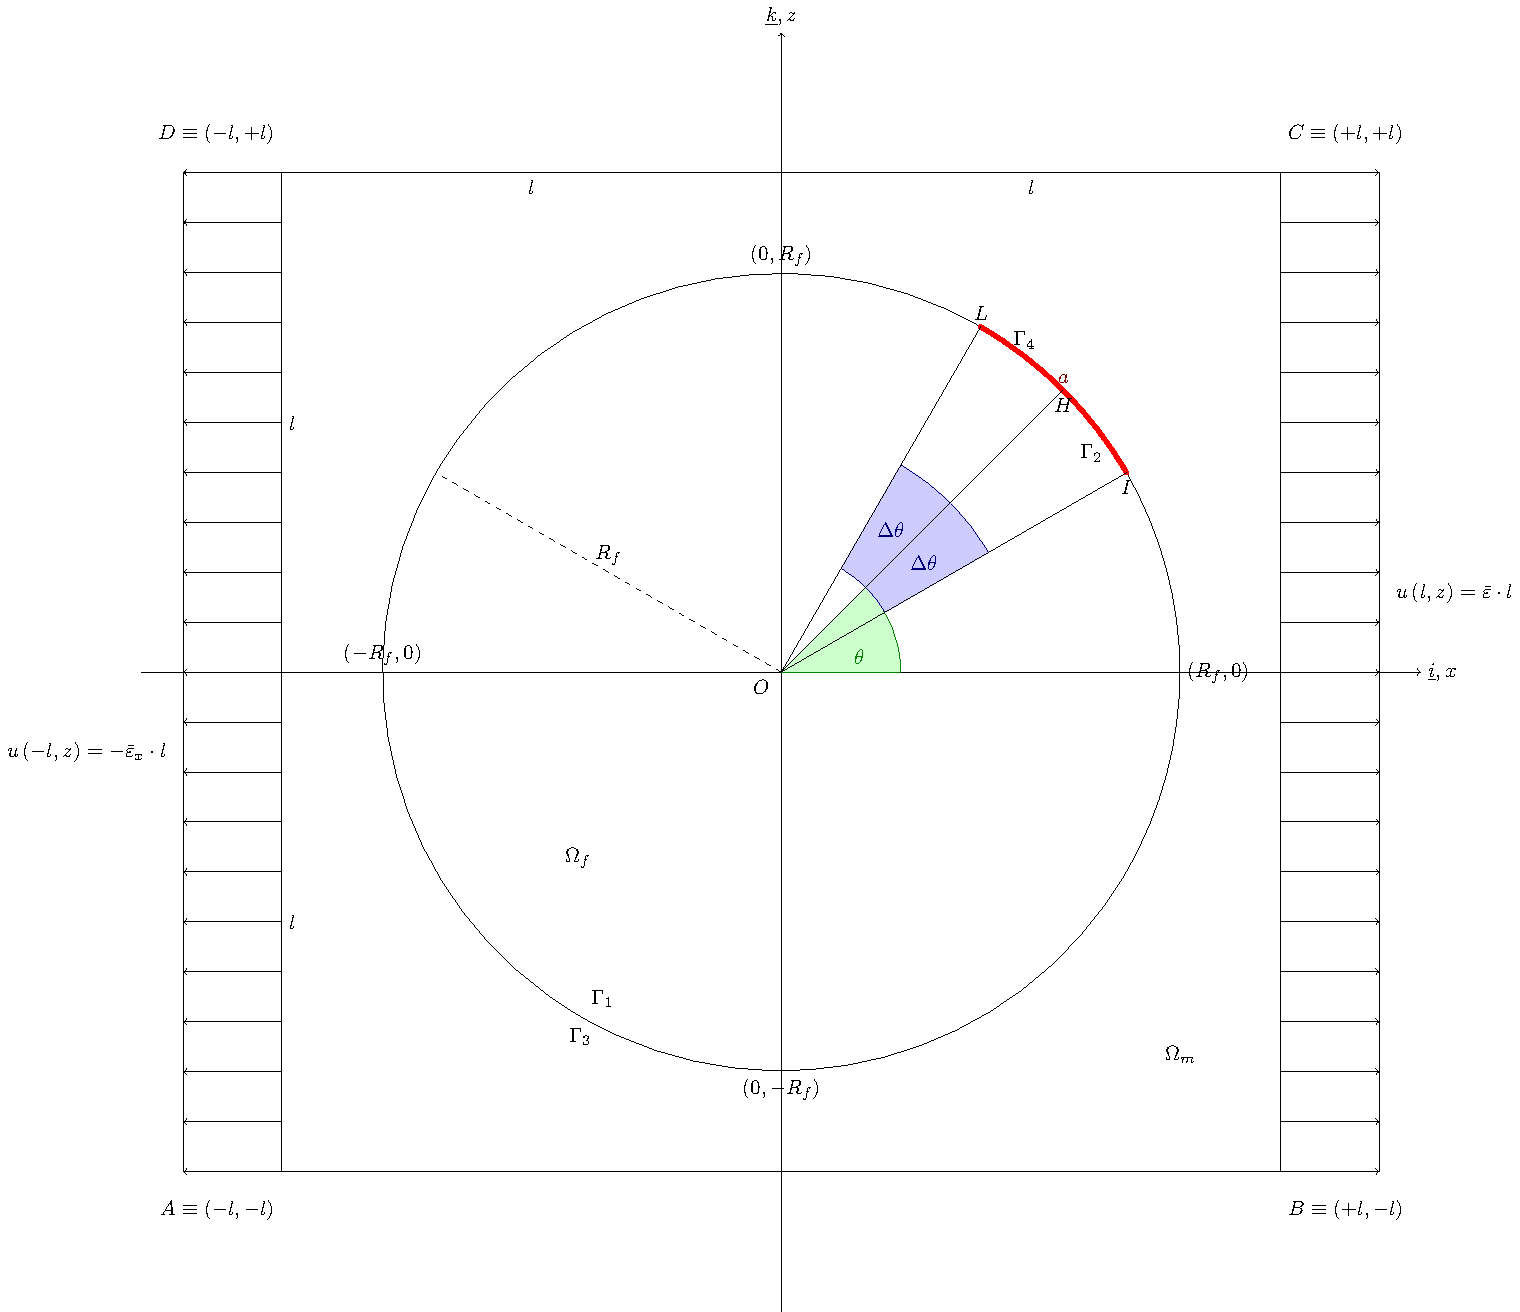
\includegraphics[height=0.7\textheight]{LEFM2DsRVEsFsDfreeBCULappAxialDispLR.pdf}
\caption{\scriptsize Simple RVE, BC: free.}
\label{fig:singleRVE-rigid}
\end{figure}
\end{frame}

\begin{frame}
\frametitle{Reference Models}
\vspace{-0.25cm}
\centering
\begin{figure}
\centering
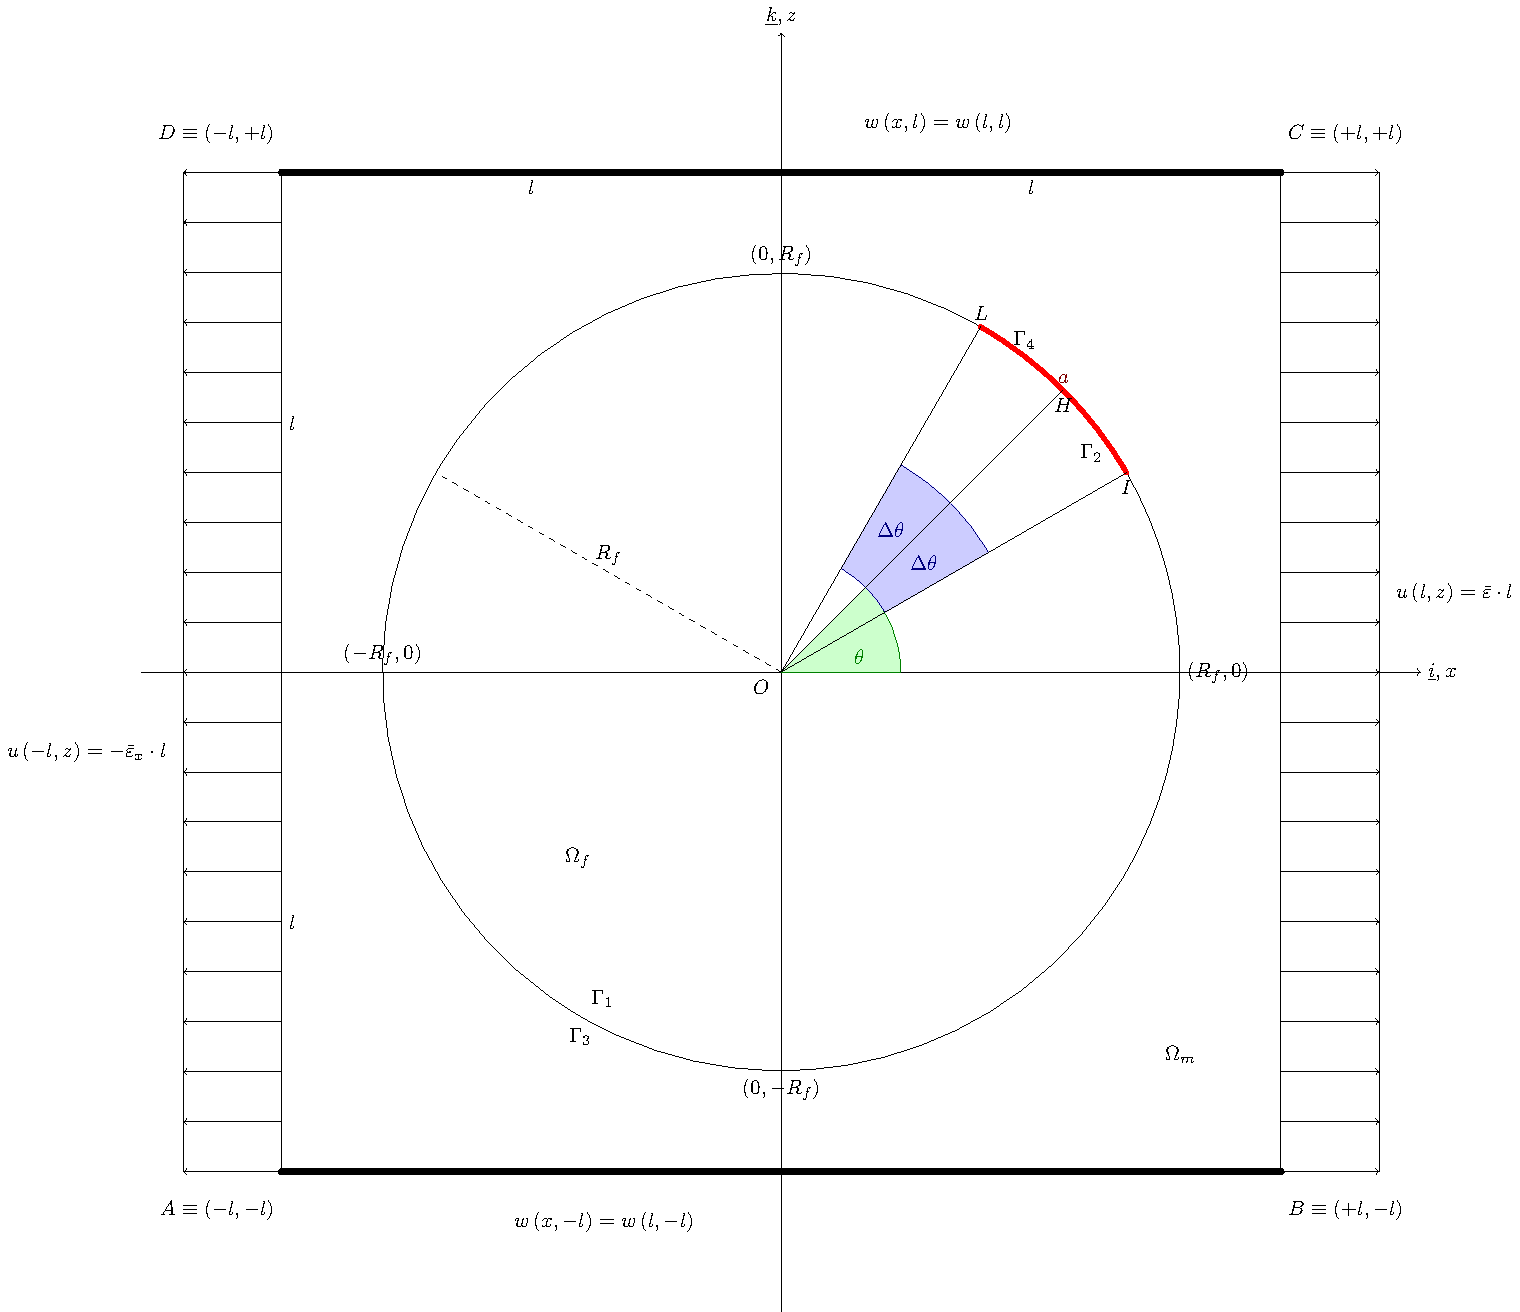
\includegraphics[height=0.7\textheight]{LEFM2DsRVEsFsDdepverdispBCULappAxialDispLR.pdf}
\caption{\scriptsize Simple RVE, BC: fixed vertical displacement.}
\label{fig:singleRVE-rigid}
\end{figure}
\end{frame}

\begin{frame}
\frametitle{Reference Models}
\vspace{-0.25cm}
\centering
\begin{figure}
\centering
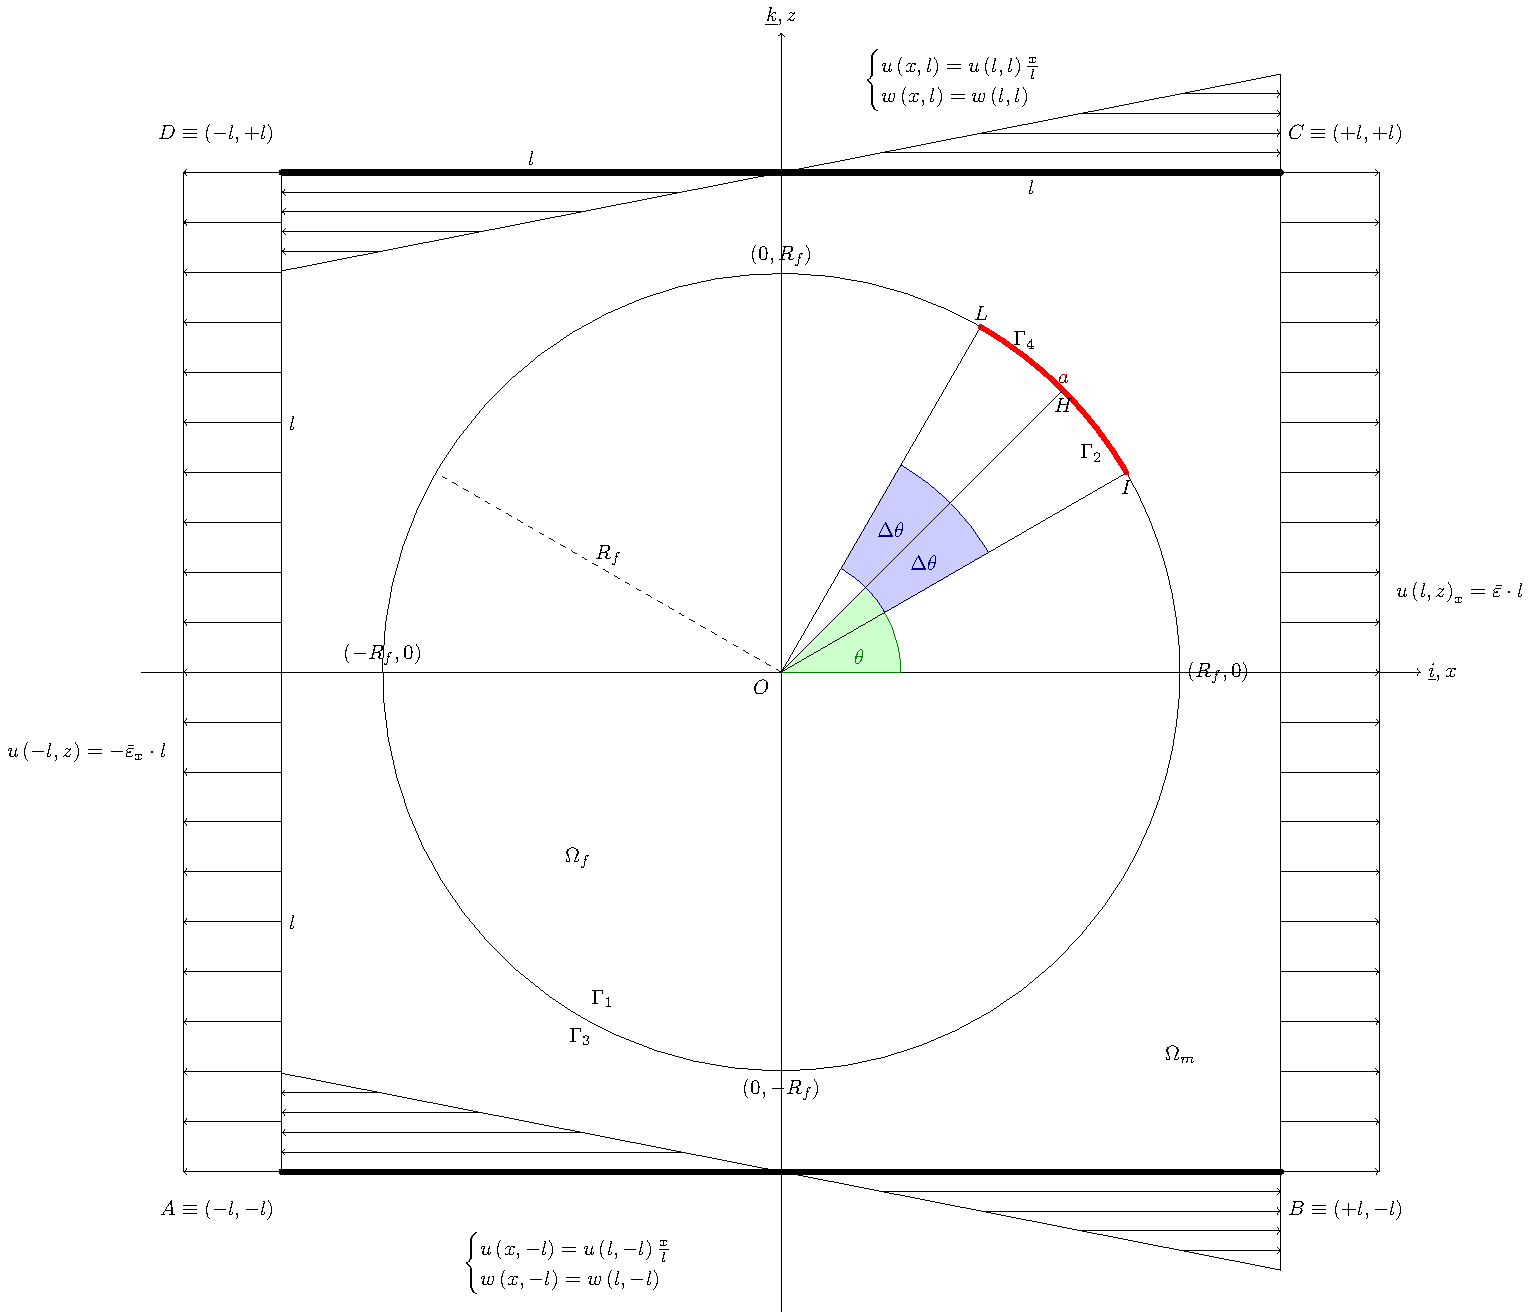
\includegraphics[height=0.7\textheight]{LEFM2DsRVEsFsDhomoBCULappAxialDispLR.pdf}
\caption{\scriptsize Simple RVE, BC: fixed vertical and homogeneous horizontal displacement.}
\label{fig:singleRVE-homo}
\end{figure}
\end{frame}

\subsection{Angular discretization}

\begin{frame}
\frametitle{Angular discretization}
\vspace{-0.7cm}
\centering
\captionsetup[figure]{font=scriptsize,labelfont=scriptsize}
\begin{figure}[!h]
\centering
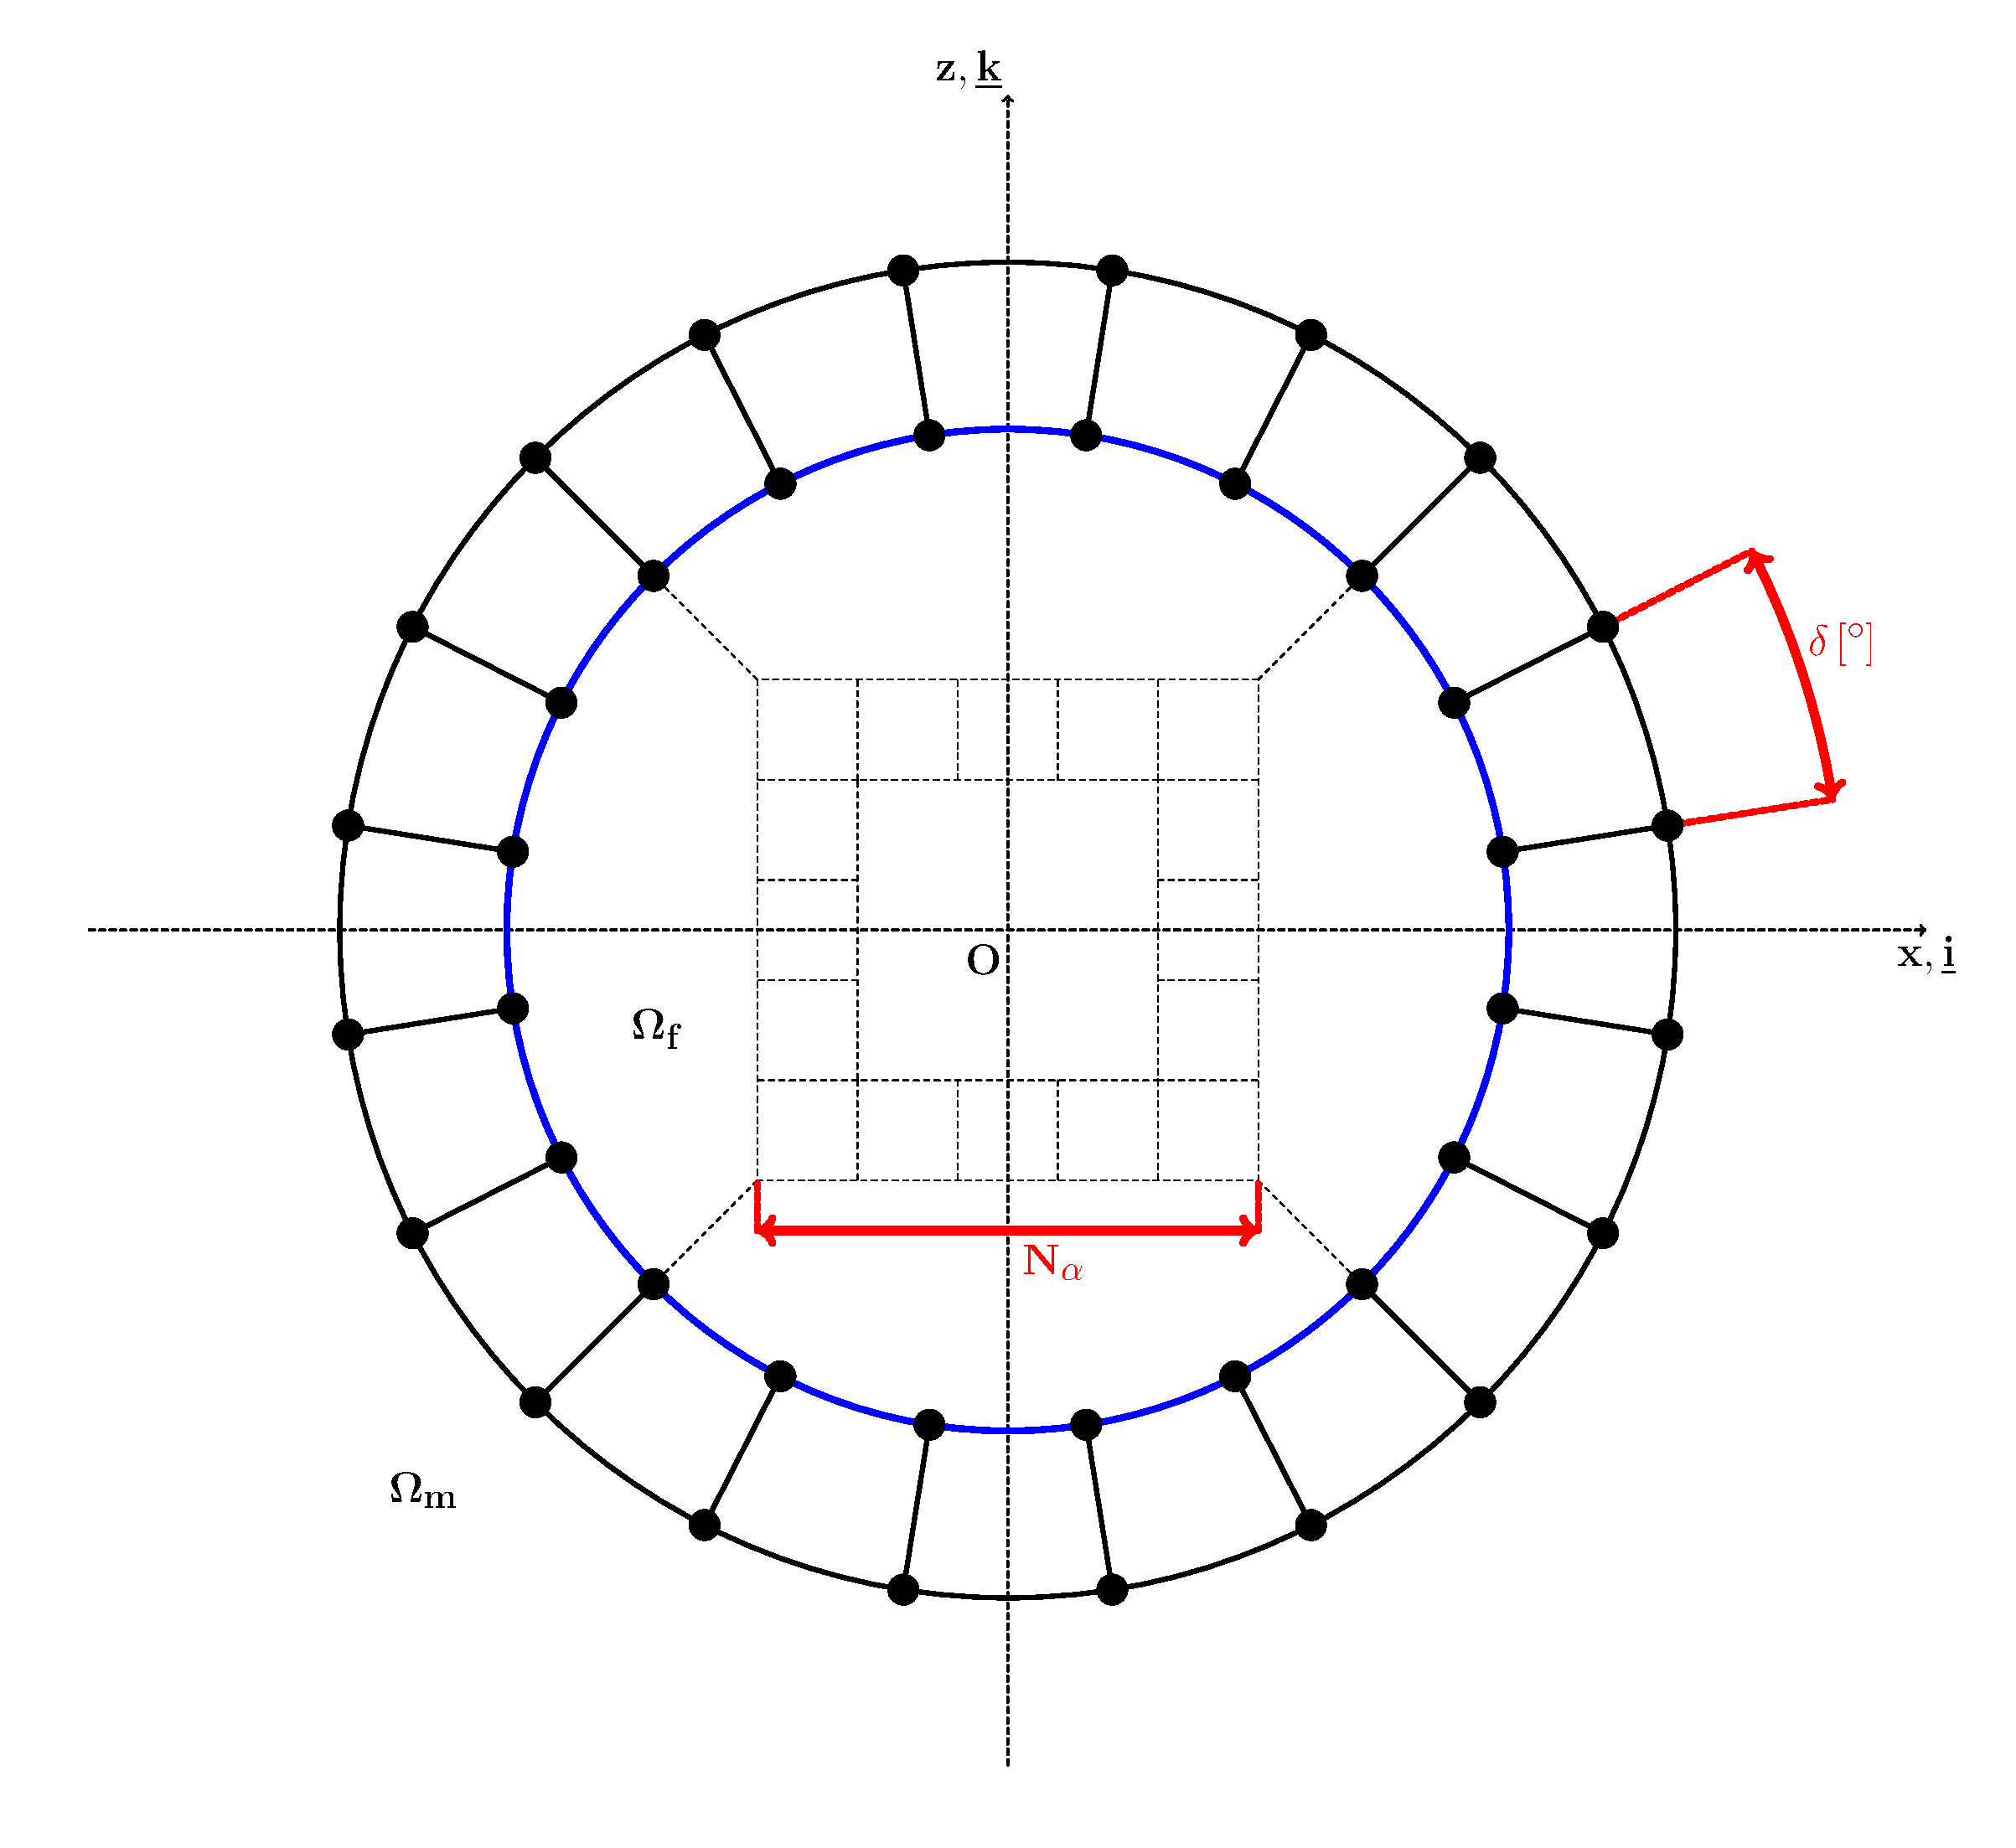
\includegraphics[height=0.7\textheight]{mesh-disc-at-interface.pdf}
  \caption{\scriptsize Angular discretization at fiber/matrix interface: $\delta=\frac{360^{\circ}}{4N_{\alpha}}$.}
  \label{fig:angu-discr-def}
\end{figure}
\end{frame}

\subsection{Material properties}

\begin{frame}
\frametitle{Material properties}
\vspace{-0.7cm}
\footnotesize
\centering
\captionsetup[figure]{font=scriptsize,labelfont=scriptsize}
\begin{table}[htbp]

  \centering
  %\caption{Single phase properties summary.}
    \begin{tabular}{cccc}

    \textbf{Material} & \textbf{$E\left[GPa\right]$}\ & \textbf{$G\left[GPa\right]$} & \textbf{$\nu\left[-\right]$} \\[3pt]
    \midrule\\[12pt]
    Glass fiber    & 70,0  & 29,2   & 0,2  \\[16pt]
    Epoxy    & 3,5    & 1,25   & 0,4  

    \end{tabular}%
  \label{tab:phaseprop}%
\end{table}%
\end{frame}

\subsection{Evaluation of $G_{0}$}
\begin{frame}
\frametitle{Evaluation of $G_{0}$}
\vspace{-0.7cm}
\footnotesize
\centering
\captionsetup[figure]{font=scriptsize,labelfont=scriptsize}
\begin{equation}
G_{0}=\pi R_{f}\sigma^{2}_{0}\frac{1+k_{m}}{8G_{m}}
\end{equation}
\begin{equation}
k_{m}=3-4\nu_{m}
\end{equation}
\begin{equation}
\sigma_{0}=\frac{E_{m}}{1-\nu^{2}_{m}}\varepsilon_{xx}
\end{equation}%
\end{frame}

\subsection{VCCT}
\begin{frame}
\frametitle{VCCT  in Forces}
\vspace{-0.5cm}
\tiny
\centering
\captionsetup[figure]{font=scriptsize,labelfont=scriptsize}
\begin{equation}
\Delta u = \left(x^{fiber, def}_{\text{1 element before crack tip}}-x^{fiber, undef}_{\text{1 element before crack tip}}\right)-\left(x^{matrix, def}_{\text{1 element before crack tip}}-x^{matrix, undef}_{\text{1 element before crack tip}}\right)
\end{equation}

\begin{equation}
\Delta w = \left(z^{fiber, def}_{\text{1 element before crack tip}}-z^{fiber, undef}_{\text{1 element before crack tip}}\right)-\left(z^{matrix, def}_{\text{1 element before crack tip}}-z^{matrix, undef}_{\text{1 element before crack tip}}\right)
\end{equation}

\begin{equation}
\beta=\arctan{\left(\frac{z^{matrix, def}_{\text{crack tip}}}{x^{matrix, def}_{\text{crack tip}}}\right)}
\end{equation}

\begin{equation}
\Delta_{r}=\cos{\left(\beta\right)}\Delta u+\sin{\left(\beta\right)}\Delta w\qquad\Delta_{\theta}=-\sin{\left(\beta\right)}\Delta u+\cos{\left(\beta\right)}\Delta w
\end{equation}

\begin{equation}
F_{r}=\cos{\left(\beta\right)}F^{reaction}_{x}+\sin{\left(\beta\right)}F^{reaction}_{z}\qquad F_{\theta}=-\sin{\left(\beta\right)}F^{reaction}_{x}+\cos{\left(\beta\right)}F^{reaction}_{z}
\end{equation}

\begin{equation}
G_{I}=\frac{1}{2}\frac{F_{r}\Delta_{r}}{R_{f}\delta}\qquad G_{II}=\frac{1}{2}\frac{F_{\theta}\Delta_{\theta}}{R_{f}\delta}\qquad b=1.0\leftrightarrow\Delta A = bR_{f}\delta
\end{equation}
\end{frame}

\begin{frame}
\frametitle{VCCT  in Stresses}
\vspace{-0.5cm}
\tiny
\centering
\captionsetup[figure]{font=scriptsize,labelfont=scriptsize}
\begin{equation}
\Delta u = \left(x^{fiber, def}_{\text{1 element before crack tip}}-x^{fiber, undef}_{\text{1 element before crack tip}}\right)-\left(x^{matrix, def}_{\text{1 element before crack tip}}-x^{matrix, undef}_{\text{1 element before crack tip}}\right)
\end{equation}

\begin{equation}
\Delta w = \left(z^{fiber, def}_{\text{1 element before crack tip}}-z^{fiber, undef}_{\text{1 element before crack tip}}\right)-\left(z^{matrix, def}_{\text{1 element before crack tip}}-z^{matrix, undef}_{\text{1 element before crack tip}}\right)
\end{equation}


\begin{equation}
\Delta_{r}=\cos{\left(\beta\right)}\Delta u+\sin{\left(\beta\right)}\Delta w\quad\Delta_{\theta}=-\sin{\left(\beta\right)}\Delta u+\cos{\left(\beta\right)}\Delta w\qquad\text{with}\quad\beta=\arctan{\left(\frac{z^{matrix, def}_{\text{crack tip}}}{x^{matrix, def}_{\text{crack tip}}}\right)}
\end{equation}

\begin{equation}
\sigma_{\left(\cdot\cdot\right)}=\frac{1}{2}\left(\sigma^{\text{element after crack tip}}_{\text{crack tip},\left(\cdot\cdot\right)}+\sigma^{\text{element before crack tip}}_{\text{crack tip},\left(\cdot\cdot\right)}\right)
\end{equation}

\begin{equation}
\sigma_{rr}=\cos^{2}{\left(\beta\right)}\sigma_{xx}+2\sin{\left(\beta\right)}\cos{\left(\beta\right)}\tau_{xz}+\sin^{2}{\left(\beta\right)}\sigma_{zz}
\end{equation}
\begin{equation}
\tau_{r\theta}=\left(\sigma_{xx}+\sigma_{zz}\right)\sin{\left(\beta\right)}\cos{\left(\beta\right)} + \tau_{xz}\left(\cos^{2}{\left(\beta\right)}-\sin^{2}{\left(\beta\right)}\right)
\end{equation}

\begin{equation}
G_{I}=\frac{1}{2}\sigma_{r}\Delta_{r}\qquad G_{II}=\frac{1}{2}\tau_{r\theta}\Delta_{\theta}\qquad \left(b=1.0\right)
\end{equation}
\end{frame}

\section{Developments \& Work Realised}

\subsection[Previous results]{Summary of previous results}

\begin{frame}
\frametitle{Summary of previous results}
\vspace{-0.25cm}
\scriptsize
\begin{list}{\Large\textcolor{green}{$\mathbf{\checkmark}$}}{}  
\item Correct global elastic response
\item Symmetric results for symmetric model
\item Correct order of magnitude of energy release rate
\item Correct trends in mode ratio: $G_{I}\uparrow\Delta\theta\downarrow$, $G_{II}\uparrow\Delta\theta\uparrow$
\item For $VF_{f}\to 0$ boundary conditions do not have effect on the result
\item Interface formulation is effectively frictionless
\end{list}
\begin{list}{\Huge\textcolor{red}{$\mathbf{\times}$}}{}  
\item No agreement with BEM results
\begin{itemize}[label=\ding{212}]
\item Overestimated energy release rate
\item Shifts of maxima of $\sim 10^{\circ}$
\end{itemize}
\end{list}
\end{frame}

\subsection[Objectives]{Summary of objectives}

\begin{frame}
\frametitle{Summary of objectives}
\vspace{-0.5cm}
\vspace{-0.5cm}
\begin{list}{$\text{\rlap{\textcolor{white}{\huge$\mathbf{\checkmark}$}}}\square$}{}  
\item Change interface formulation
\item To test new formulations, create model of debond between two infinite half-planes of different isotropic materials
\end{list}
\end{frame}

\subsection{Work realised \& Follow-Up Actions}

\begin{frame}
\frametitle{Notation}
\vspace{-0.5cm}
\scriptsize
\begin{list}{$\text{\rlap{\textcolor{white}{\huge$\mathbf{\checkmark}$}}}\square$}{}  
\item Planned/proposed action
\end{list}
\begin{list}{$\text{\rlap{\textcolor{green}{\huge$\mathbf{\checkmark}$}}}\square$}{}
\item Task completed
\end{list}
\begin{list}{$\text{\rlap{\textcolor{orange}{\huge$\mathbf{\checkmark}$}}}\square$}{}  
\item Task in progress
\end{list}
\end{frame}

\begin{frame}
\frametitle{Work realised \& Follow-Up Actions}
\vspace{-0.5cm}
\scriptsize
\begin{list}{$\text{\rlap{\textcolor{white}{\huge$\mathbf{\checkmark}$}}}\square$}{}  
\item Interface formulations (2/9)
\begin{itemize}[label=\ding{212}]
\item (Old formulation) 2 surfaces: $\text{fibre surface}=\Gamma_{1}+\Gamma_{2}$ et $\text{matrix surface}=\Gamma_{3}+\Gamma_{4}$ with interaction $^{*}CONTACT$ and $^{*}DEBOND$, SMALL-SLIDING with SURFACE TO SURFACE DEFINITION (with $^{*}DEBOND$ in Abaqus/Standard crack surfaces are rigidly bonded when uncracked)
\end{itemize}
\begin{list}{$\text{\rlap{\textcolor{green}{\huge$\mathbf{\checkmark}$}}}\square$}{}  
\item 4 surfaces: $\Gamma_{1}$ WITHOUT crack tip, $\Gamma_{2}$ WITH crack tip, $\Gamma_{3}$ WITHOUT crack tip and $\Gamma_{4}$ WITH crack tip, interaction $*TIE$ between $\Gamma_{1}$ and $\Gamma_{3}$, interaction $^{*}CONTACT$ and $^{*}DEBOND$ between $\Gamma_{2}$ and $\Gamma_{4}$, SMALL-SLIDING with SURFACE TO SURFACE DEFINITION
\begin{list}{$\text{\rlap{\textcolor{green}{\huge$\mathbf{\checkmark}$}}}\square$}{}
\item Development of preprocessor
\item FEM model creation
\item Parametric simulation
\item Analysis of results
\end{list}
\end{list}
\end{list}
\end{frame}

\begin{frame}
\frametitle{Work realised \& Follow-Up Actions}
\vspace{-0.5cm}
\scriptsize
\begin{list}{$\text{\rlap{\textcolor{white}{\huge$\mathbf{\checkmark}$}}}\square$}{}  
\item Interface formulations (3/9)
\begin{list}{$\text{\rlap{\textcolor{green}{\huge$\mathbf{\checkmark}$}}}\square$}{}  
\item 2 surfaces: $\Gamma_{2}$ WITH crack tip and $\Gamma_{4}$ WITH crack tip, interaction $^{*}CONTACT$ et $^{*}DEBOND$ between  $\Gamma_{2}$ and $\Gamma_{4}$, interaction $^{*}MPC\ TIE$ between \textit{nodes} of $\Gamma_{1}$ and $\Gamma_{3}$, SMALL-SLIDING with SURFACE TO SURFACE DEFINITION
\begin{list}{$\text{\rlap{\textcolor{green}{\huge$\mathbf{\checkmark}$}}}\square$}{}
\item Development of preprocessor
\item FEM model creation
\item Parametric simulation
\item Analysis of results
\end{list}
\end{list}
\end{list}
\end{frame}

\begin{frame}
\frametitle{Work realised \& Follow-Up Actions}
\vspace{-0.5cm}
\scriptsize
\begin{list}{$\text{\rlap{\textcolor{white}{\huge$\mathbf{\checkmark}$}}}\square$}{}  
\item Interface formulations (4/9)
\begin{list}{$\text{\rlap{\textcolor{green}{\huge$\mathbf{\checkmark}$}}}\square$}{}  
\item  4 surfaces: $\Gamma_{1}$ WITH crack tip, $\Gamma_{2}$ WITHOUT crack tip, $\Gamma_{3}$ WITH crack tip and $\Gamma_{4}$ WITHOUT crack tip, interaction $^{*}TIE$ between  $\Gamma_{1}$ and $\Gamma_{3}$, interaction $^{*}CONTACT$ between  $\Gamma_{2}$ and $\Gamma_{4}$
\begin{list}{$\text{\rlap{\textcolor{green}{\huge$\mathbf{\checkmark}$}}}\square$}{}
\item Development of preprocessor
\item FEM model creation
\item Parametric simulation
\item Implementation of VCCT (in stresses) procedure in the postprocessor
\item Analysis of results
\end{list}
\end{list}
\end{list}
\end{frame}

\begin{frame}
\frametitle{Work realised \& Follow-Up Actions}
\vspace{-0.5cm}
\scriptsize
\begin{list}{$\text{\rlap{\textcolor{white}{\huge$\mathbf{\checkmark}$}}}\square$}{}  
\item Interface formulations (5/9)
\begin{list}{$\text{\rlap{\textcolor{green}{\huge$\mathbf{\checkmark}$}}}\square$}{}  
\item  2 surfaces: $\Gamma_{2}$ WITHOUT crack tip and $\Gamma_{4}$ WITHOUT crack tip, interaction $^{*}CONTACT$ between  $\Gamma_{2}$ and $\Gamma_{4}$, interaction $^{*}MPC\ TIE$ between \textit{nodes} of $\Gamma_{1}$ and $\Gamma_{3}$
\begin{list}{$\text{\rlap{\textcolor{green}{\huge$\mathbf{\checkmark}$}}}\square$}{}
\item Development of preprocessor
\item FEM model creation
\item Parametric simulation
\item Implementation of VCCT (in stresses) procedure in the postprocessor
\item Analysis of results
\end{list}
\end{list}
\end{list}
\end{frame}

\begin{frame}
\frametitle{Work realised \& Follow-Up Actions}
\vspace{-0.5cm}
\scriptsize
\begin{list}{$\text{\rlap{\textcolor{white}{\huge$\mathbf{\checkmark}$}}}\square$}{}  
\item Interface formulations (6/9)
\begin{list}{$\text{\rlap{\textcolor{green}{\huge$\mathbf{\checkmark}$}}}\square$}{}  
\item  2 surfaces: $\Gamma_{2}$ WITHOUT crack tip and $\Gamma_{4}$ WITHOUT crack tip, interaction $^{*}CONTACT$ between  $\Gamma_{2}$ and $\Gamma_{4}$, interaction $^{*}EQUATION$ between \textit{nodes} of $\Gamma_{1}$ and $\Gamma_{3}$ with \textit{dummy node} to measure reaction force
\begin{list}{$\text{\rlap{\textcolor{green}{\huge$\mathbf{\checkmark}$}}}\square$}{}  
\item Development of preprocessor
\item FEM model creation
\item Parametric simulation
\item Implementation of VCCT (in forces) procedure in the postprocessor
\item Analysis of results
\end{list}
\end{list}
\end{list}
\end{frame}

\begin{frame}
\frametitle{Work realised \& Follow-Up Actions}
\vspace{-0.5cm}
\scriptsize
\begin{list}{$\text{\rlap{\textcolor{white}{\huge$\mathbf{\checkmark}$}}}\square$}{}  
\item Interface formulations (7/9)
\begin{list}{$\text{\rlap{\textcolor{green}{\huge$\mathbf{\checkmark}$}}}\square$}{}  
\item  2 surfaces: $\Gamma_{2}$WITHOUT crack tip and $\Gamma_{4}$ WITHOUT crack tip, interaction $^{*}CONTACT$ between  $\Gamma_{2}$ and $\Gamma_{4}$, interaction $^{*}CONN2D2\ TIE$ between \textit{nodes} of $\Gamma_{1}$ and $\Gamma_{3}$
\begin{list}{$\text{\rlap{\textcolor{green}{\huge$\mathbf{\checkmark}$}}}\square$}{}  
\item Development of preprocessor
\item FEM model creation
\item Parametric simulation
\item Implementation of VCCT (in forces) procedure in the postprocessor
\item Analysis of results
\end{list}
\end{list}
\end{list}
\end{frame}

\begin{frame}
\frametitle{Work realised \& Follow-Up Actions}
\vspace{-0.5cm}
\scriptsize
\begin{list}{$\text{\rlap{\textcolor{white}{\huge$\mathbf{\checkmark}$}}}\square$}{}  
\item Interface formulations (8/9)
\begin{list}{$\text{\rlap{\textcolor{orange}{\huge$\mathbf{\checkmark}$}}}\square$}{}  
\item  2 surfaces: $\text{fibre surface}=\Gamma_{1}+\Gamma_{2}$ et $\text{matrix surface}=\Gamma_{3}+\Gamma_{4}$ with interaction $^{*}CONTACT$ and $^{*}DEBOND$, FINITE SLIDING with NODE TO SURFACE DEFINITION (with $^{*}DEBOND$ in Abaqus/Standard crack surfaces are rigidly bonded when uncracked)
\begin{list}{$\text{\rlap{\textcolor{green}{\huge$\mathbf{\checkmark}$}}}\square$}{}  
\item Development of preprocessor
\item FEM model creation
\end{list}
\begin{list}{$\text{\rlap{\textcolor{orange}{\huge$\mathbf{\checkmark}$}}}\square$}{}
\item Parametric simulation
\end{list}
\begin{list}{$\text{\rlap{\textcolor{white}{\huge$\mathbf{\checkmark}$}}}\square$}{}
\item Analysis of results
\end{list}
\end{list}
\end{list}
\end{frame}

\begin{frame}
\frametitle{Work realised \& Follow-Up Actions}
\vspace{-0.5cm}
\scriptsize
\begin{list}{$\text{\rlap{\textcolor{white}{\huge$\mathbf{\checkmark}$}}}\square$}{}  
\item Interface formulations (9/9)
\begin{list}{$\text{\rlap{\textcolor{white}{\huge$\mathbf{\checkmark}$}}}\square$}{}  
\item  2 surfaces: $\text{fibre surface}=\Gamma_{1}+\Gamma_{2}$ et $\text{matrix surface}=\Gamma_{3}+\Gamma_{4}$ with interaction $^{*}CONTACT$ and $^{*}DEBOND$, SMALL SLIDING with NODE TO SURFACE DEFINITION (with $^{*}DEBOND$ in Abaqus/Standard crack surfaces are rigidly bonded when uncracked)
\begin{list}{$\text{\rlap{\textcolor{white}{\huge$\mathbf{\checkmark}$}}}\square$}{}  
\item Development of preprocessor
\item FEM model creation
\item Parametric simulation
\item Analysis of results
\end{list}
\end{list}
\end{list}
\end{frame}

\begin{frame}
\frametitle{Work realised \& Follow-Up Actions}
\vspace{-0.5cm}
\scriptsize
\begin{list}{$\text{\rlap{\textcolor{white}{\huge$\mathbf{\checkmark}$}}}\square$}{}  
\item To test new formulations, create model of debond between two infinite half-planes of different isotropic materials
\begin{list}{$\text{\rlap{\textcolor{orange}{\huge$\mathbf{\checkmark}$}}}\square$}{} 
\item Full model
\begin{list}{$\text{\rlap{\textcolor{green}{\huge$\mathbf{\checkmark}$}}}\square$}{}
\item Development of preprocessor
\item FEM model creation and verification
\item Parametric simulation
\end{list}
\begin{list}{$\text{\rlap{\textcolor{orange}{\huge$\mathbf{\checkmark}$}}}\square$}{}
\item Implementation of VCCT procedure in the postprocessor
\end{list}
\begin{list}{$\text{\rlap{\textcolor{white}{\huge$\mathbf{\checkmark}$}}}\square$}{}
\item Analysis of results
\end{list}
\end{list}
\end{list}
\end{frame}

\begin{frame}
\frametitle{Work realised \& Follow-Up Actions}
\vspace{-0.5cm}
\scriptsize
\begin{list}{$\text{\rlap{\textcolor{white}{\huge$\mathbf{\checkmark}$}}}\square$}{}  
\item To test new formulations, create model of debond between two infinite half-planes of different isotropic materials
\begin{list}{$\text{\rlap{\textcolor{orange}{\huge$\mathbf{\checkmark}$}}}\square$}{} 
\item Symmetric model
\begin{list}{$\text{\rlap{\textcolor{green}{\huge$\mathbf{\checkmark}$}}}\square$}{}
\item Development of preprocessor
\end{list}
\begin{list}{$\text{\rlap{\textcolor{orange}{\huge$\mathbf{\checkmark}$}}}\square$}{}
\item FEM model creation and verification
\end{list}
\begin{list}{$\text{\rlap{\textcolor{white}{\huge$\mathbf{\checkmark}$}}}\square$}{}
\item Parametric simulation
\item Implementation of VCCT procedure in the postprocessor
\item Analysis of results
\end{list}
\end{list}
\end{list}
\end{frame}

\subsection{Results}

\begin{frame}
\frametitle{Results}
\vspace{-0.7cm}
\centering
\captionsetup[figure]{font=scriptsize,labelfont=scriptsize}
\begin{figure}[!h]
\centering
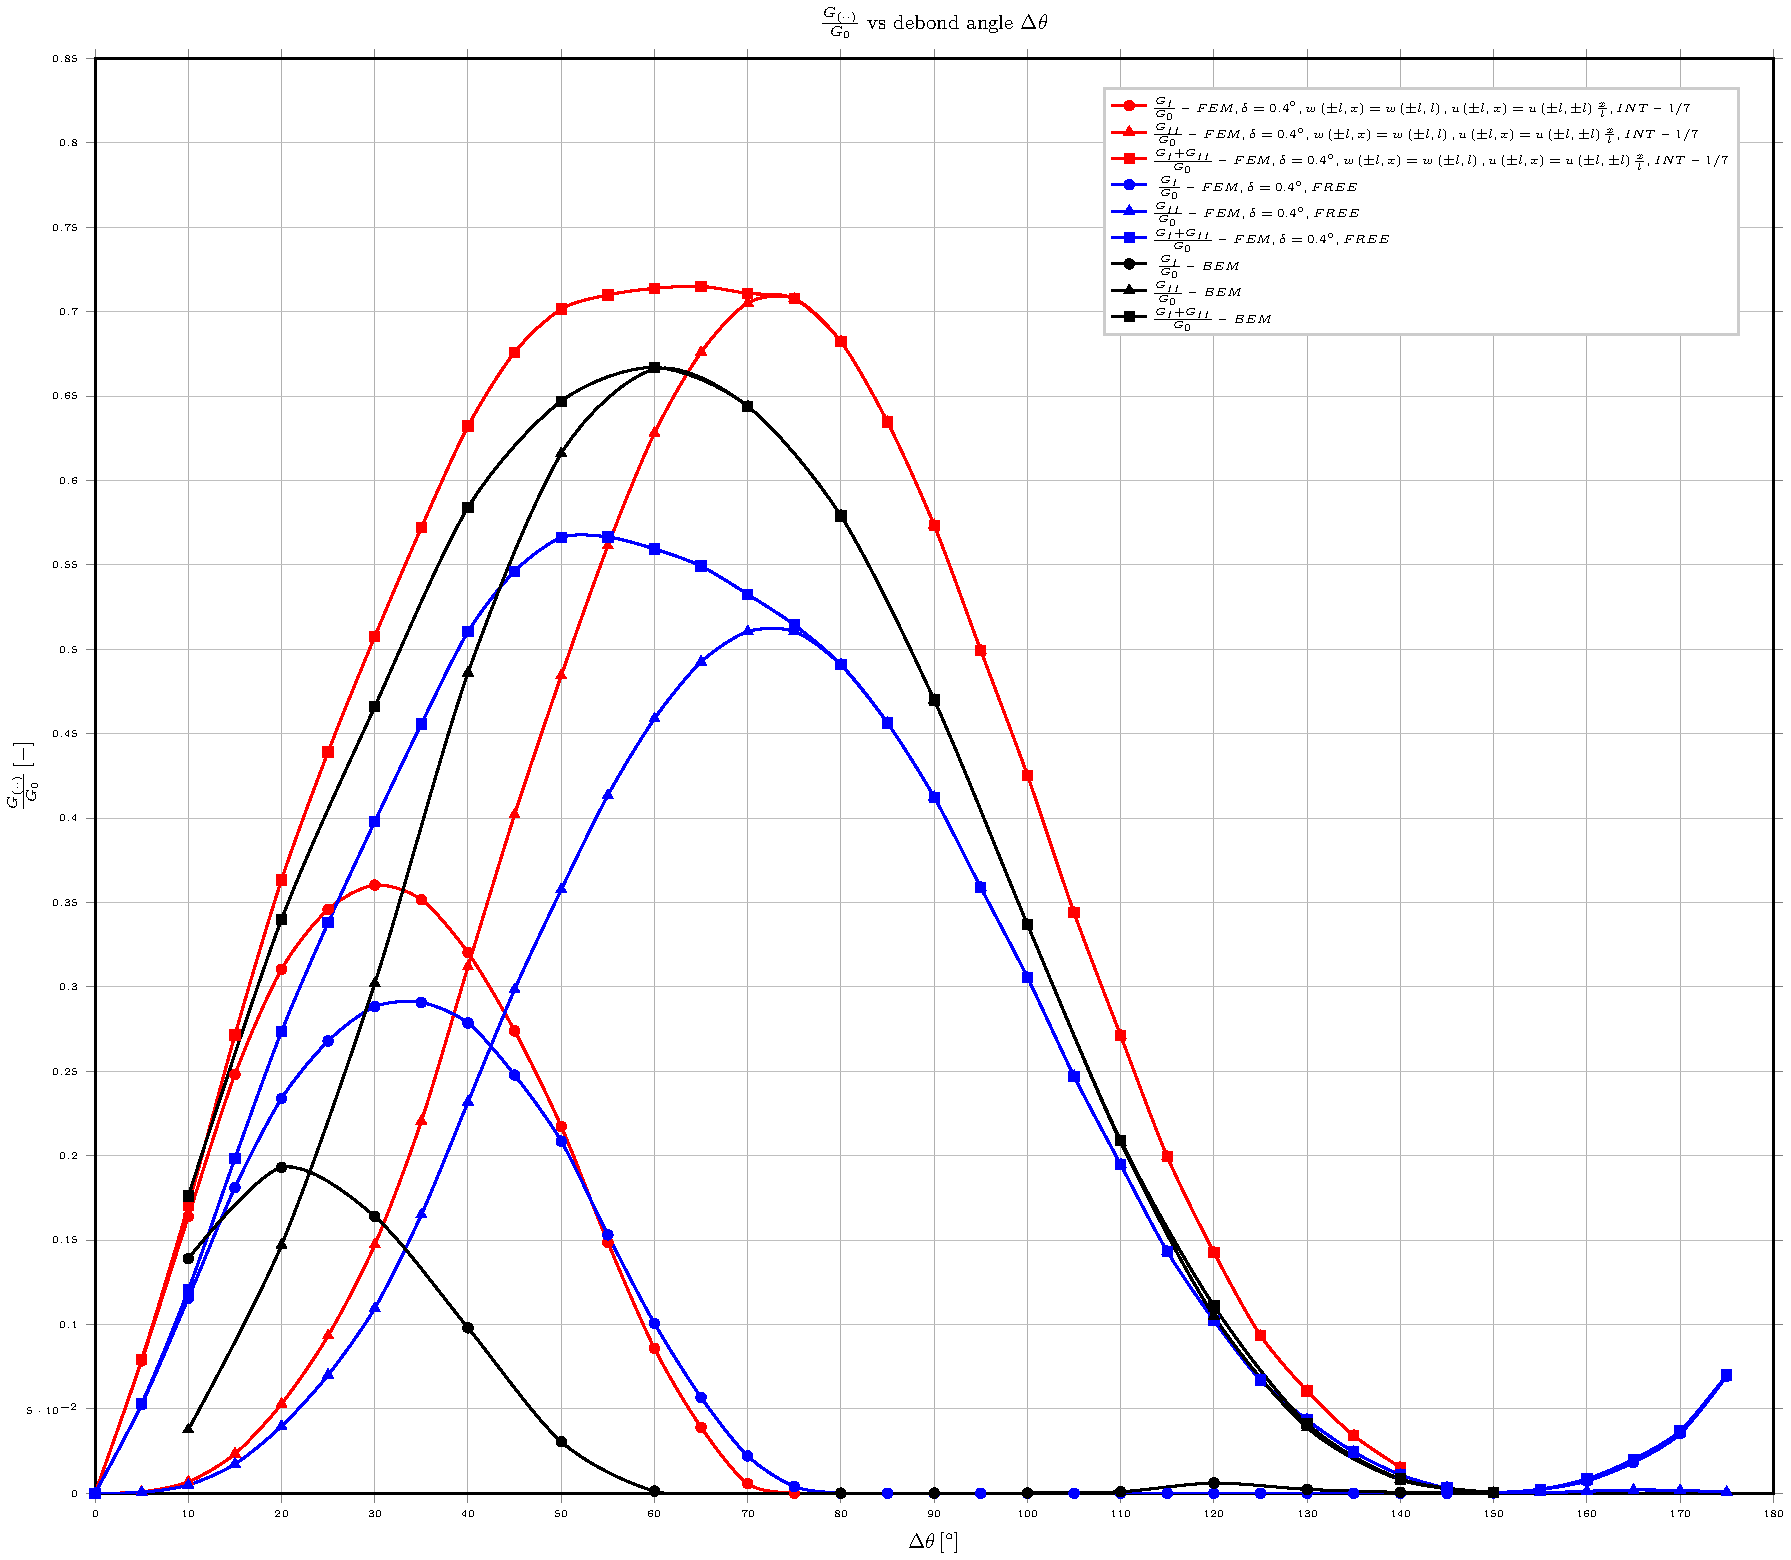
\includegraphics[height=0.7\textheight]{2017-04-29_AbqRunSummary_GsoverG0_FEM-BEM-comparison.pdf}
  \caption{\scriptsize Interface formulation 2/9, in blue.}
  \label{fig:res1}
\end{figure}
\end{frame}

\begin{frame}
\frametitle{Results}
\vspace{-0.7cm}
\centering
\captionsetup[figure]{font=scriptsize,labelfont=scriptsize}
\begin{figure}[!h]
\centering
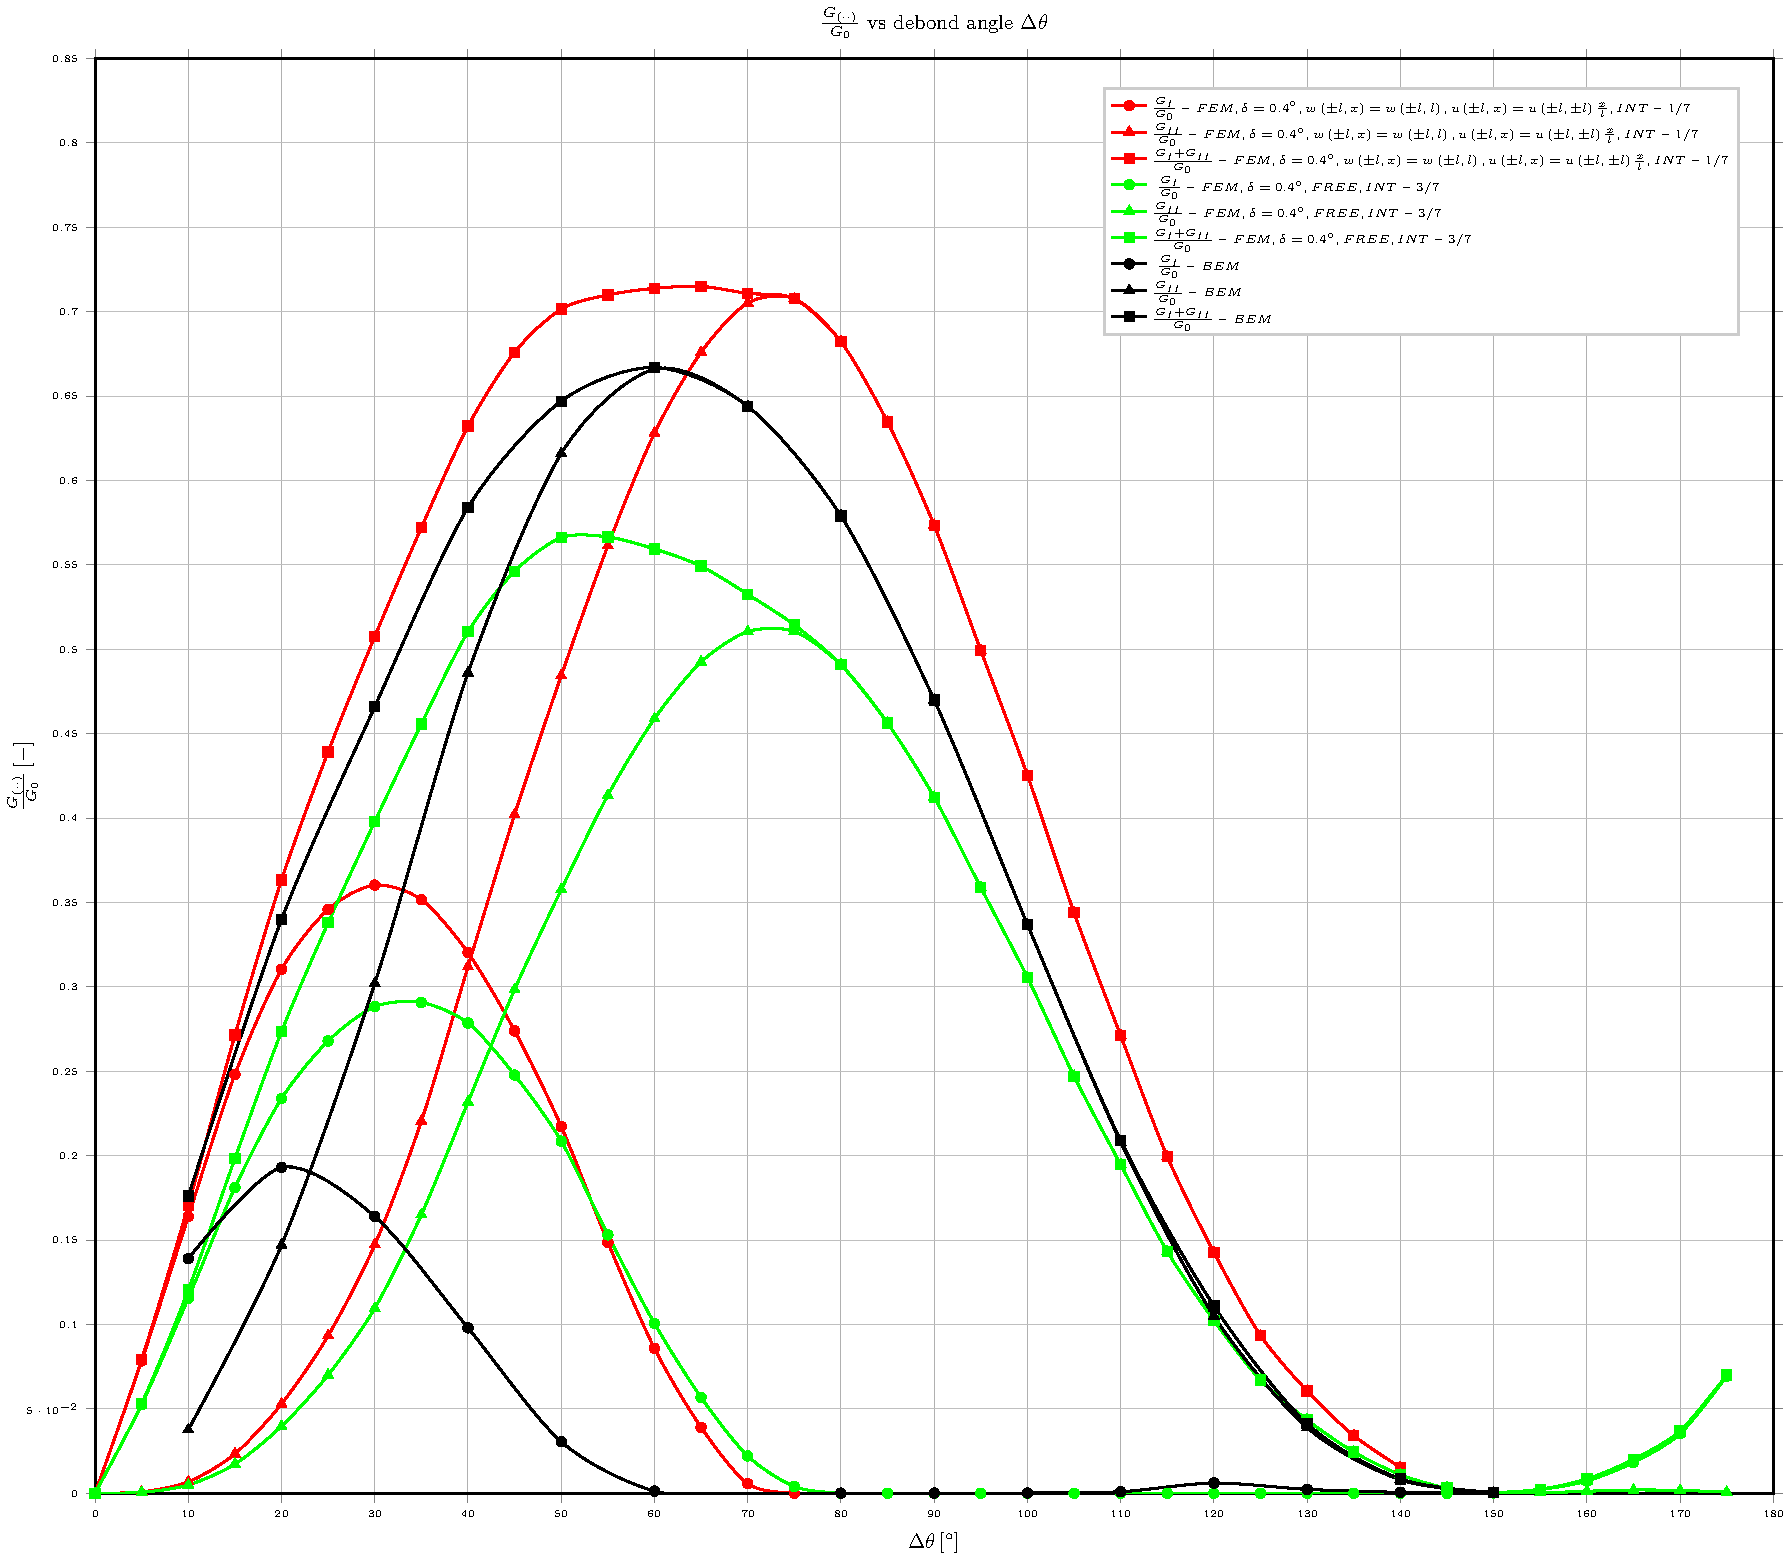
\includegraphics[height=0.7\textheight]{2017-05-03_AbqRunSummary_GsoverG0_FEM-BEM-comparison.pdf}
  \caption{\scriptsize Interface formulation 3/9, in green.}
  \label{fig:res2}
\end{figure}
\end{frame}

\begin{frame}
\frametitle{Results}
\vspace{-0.7cm}
\centering
\captionsetup[figure]{font=scriptsize,labelfont=scriptsize}
\begin{figure}[!h]
\centering
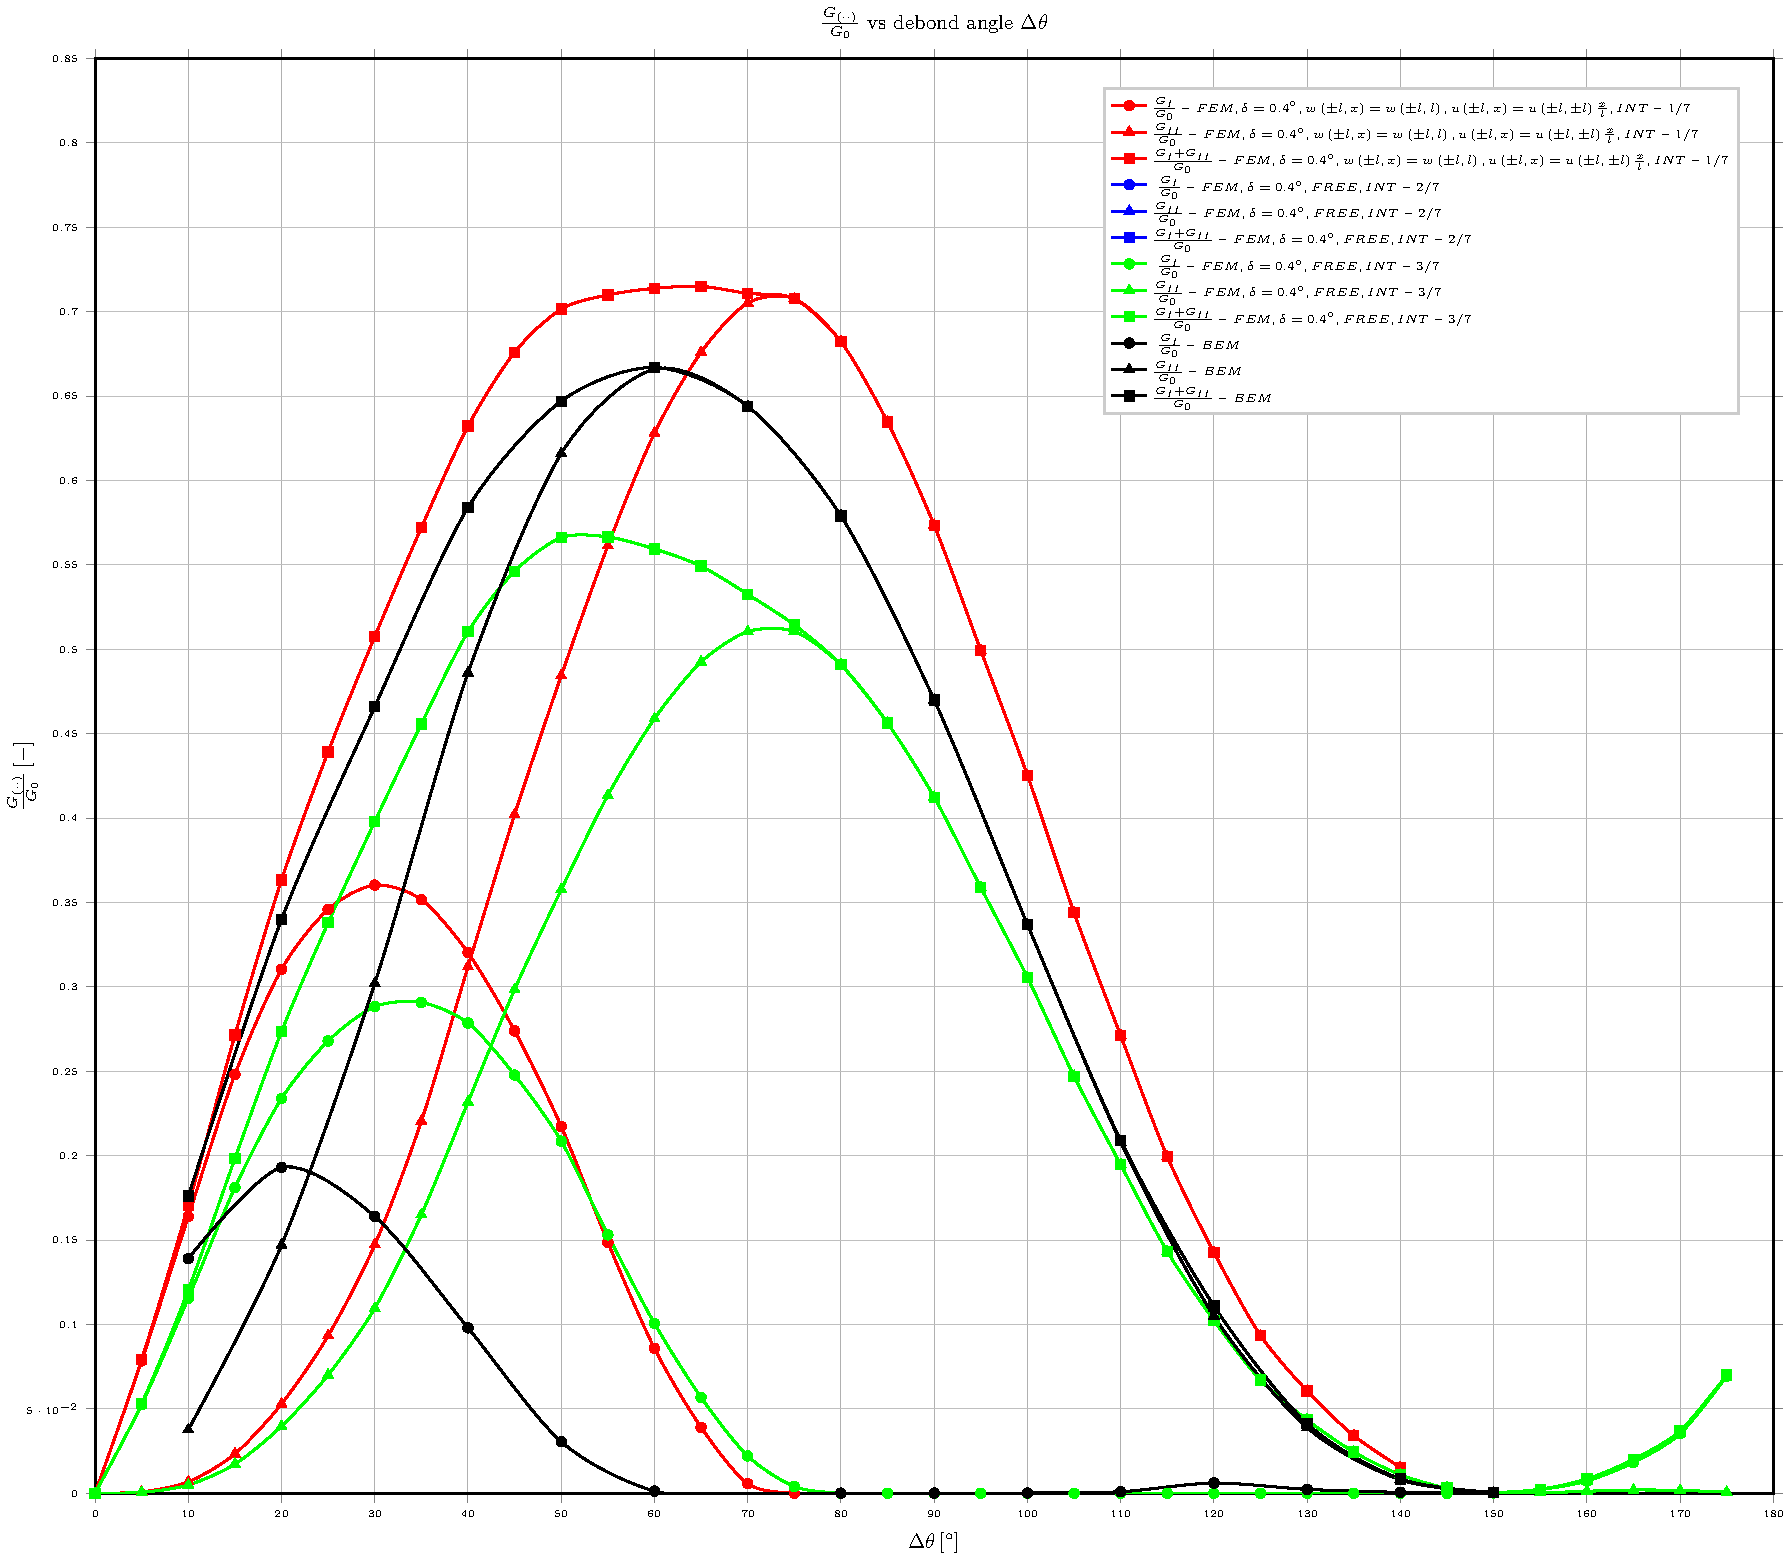
\includegraphics[height=0.7\textheight]{2017-04-29_05-03_AbqRunSummary_GsoverG0_FEM-BEM-comparison.pdf}
  \caption{\scriptsize Interface formulations 2/9 and 3/9, respectively in green and blue.}
  \label{fig:res3}
\end{figure}
\end{frame}

\begin{frame}
\frametitle{Results}
\vspace{-0.7cm}
\centering
\captionsetup[figure]{font=scriptsize,labelfont=scriptsize}
\begin{figure}[!h]
\centering
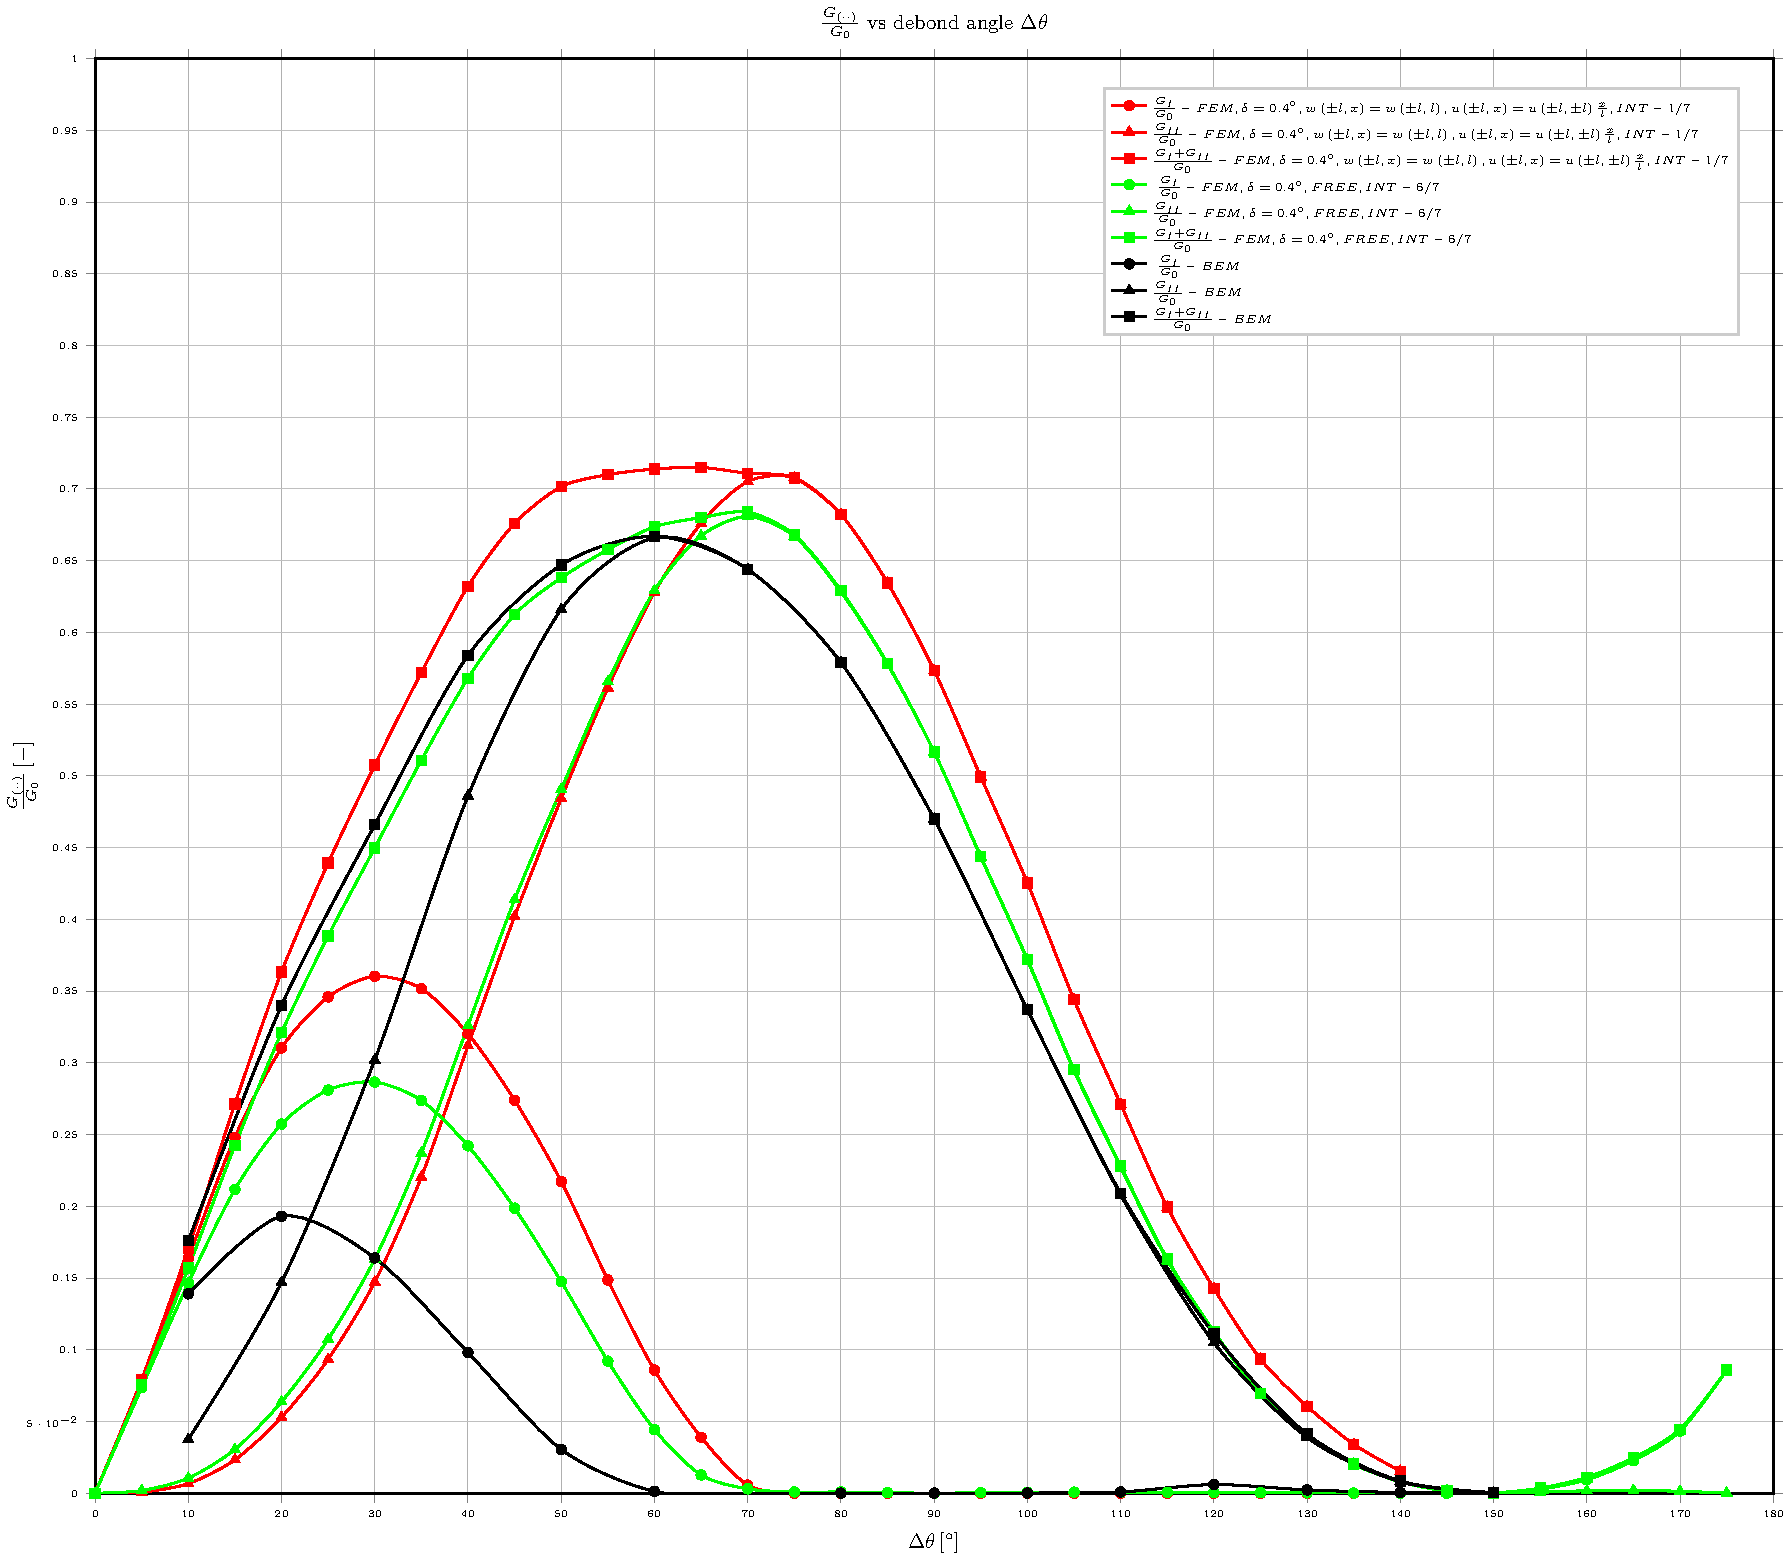
\includegraphics[height=0.7\textheight]{2017-06-01_AbqRunSummary_GsoverG0_FEM-BEM-comparison.pdf}
  \caption{\scriptsize Interface formulation 6/9, in green.}
  \label{fig:res4}
\end{figure}
\end{frame}

\begin{frame}
\frametitle{Results}
\vspace{-0.7cm}
\centering
\captionsetup[figure]{font=scriptsize,labelfont=scriptsize}
\begin{figure}[!h]
\centering
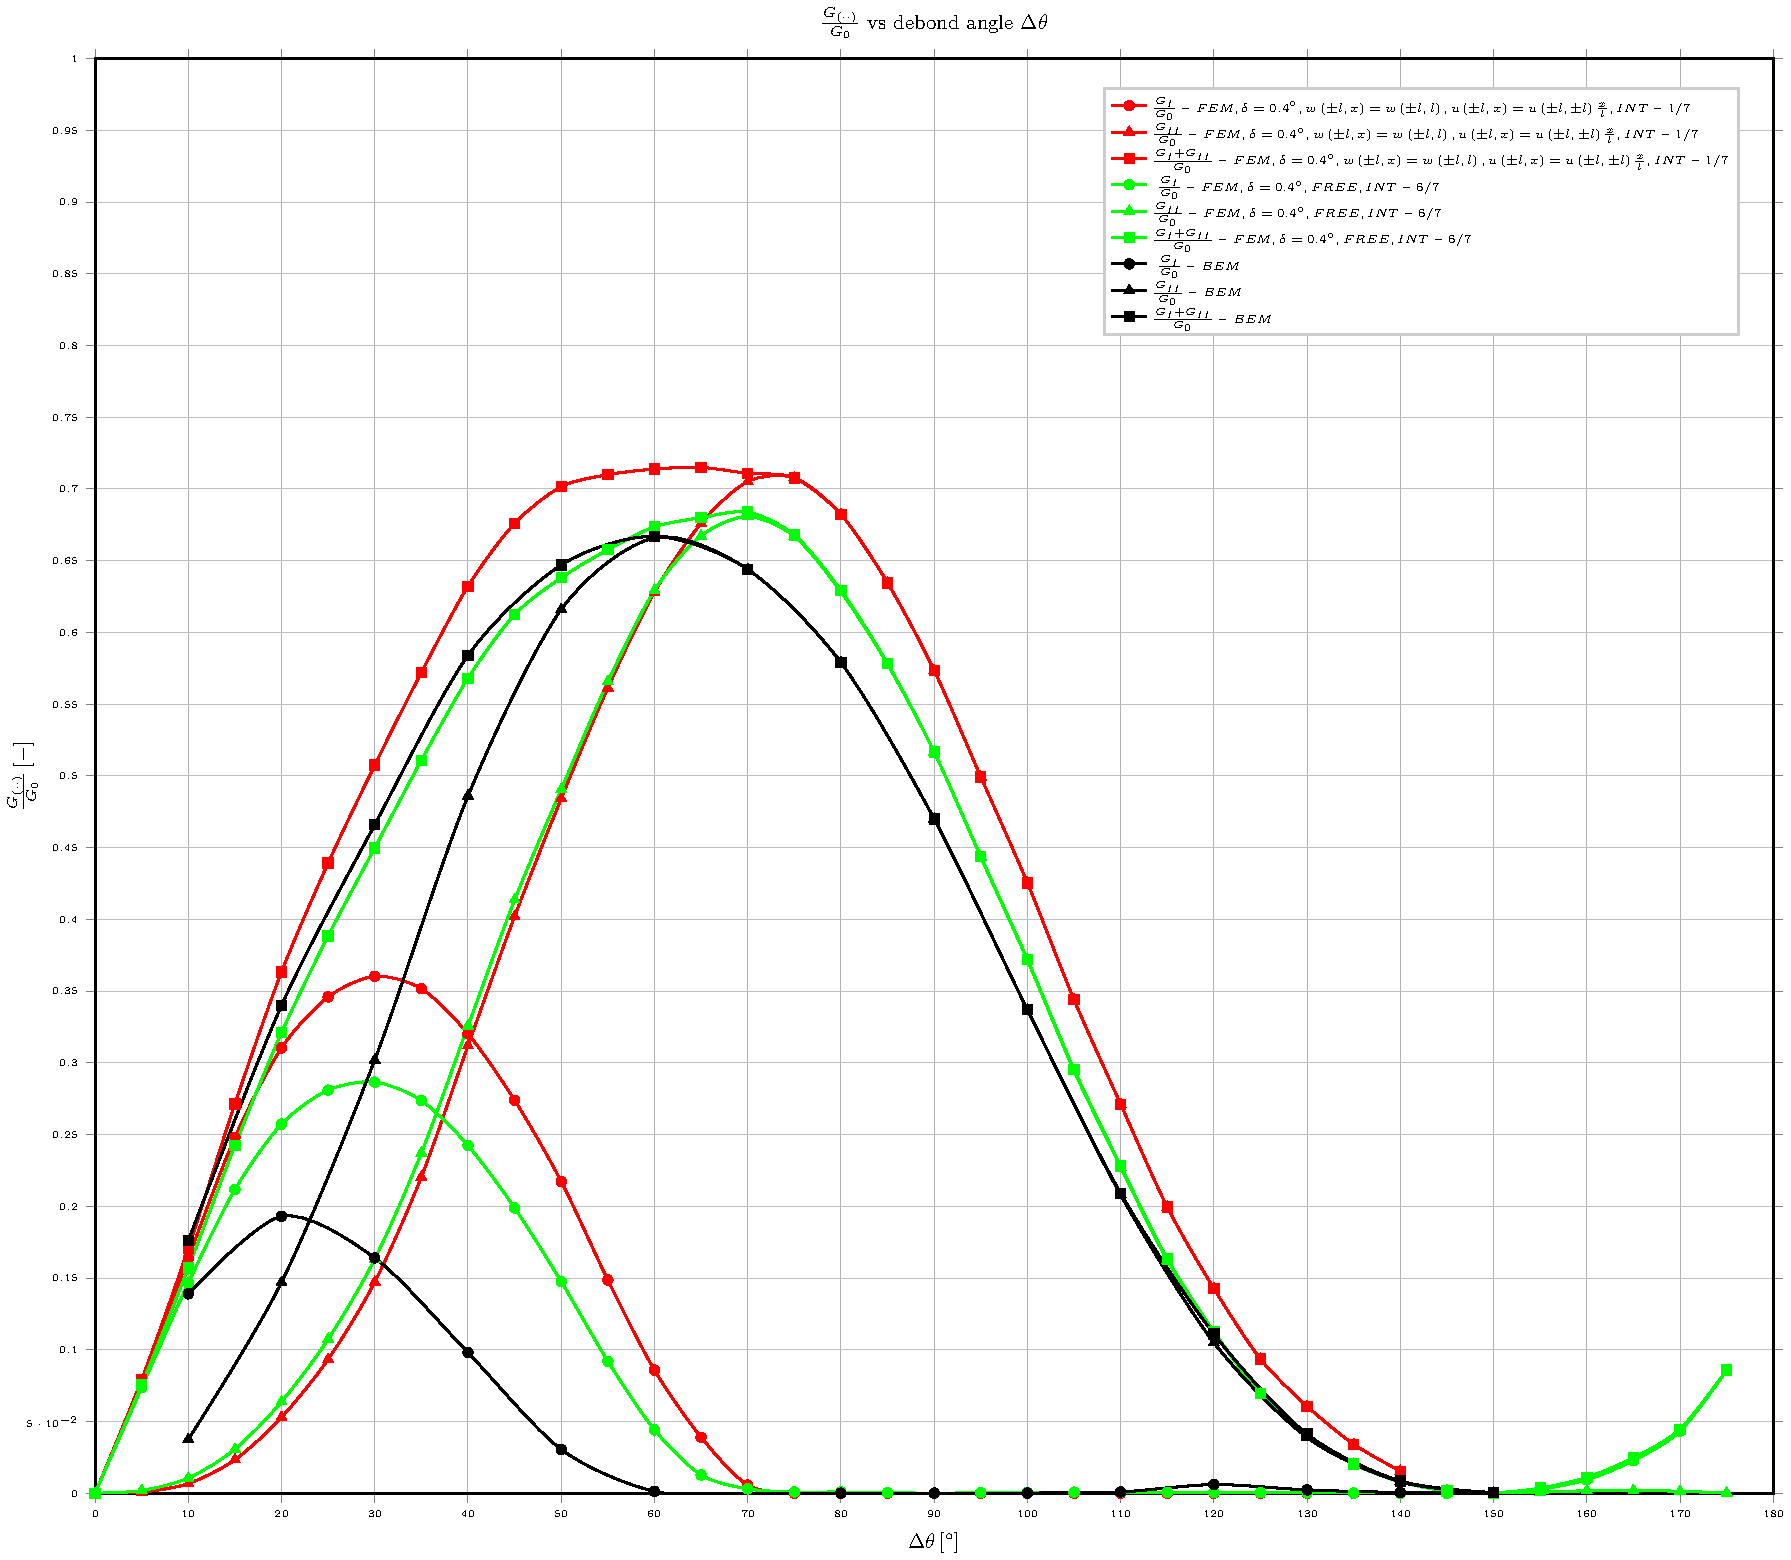
\includegraphics[height=0.7\textheight]{2017-06-01_AbqRunSummary_GsoverG0_FEM-ConnCRF-BEM-comparison.pdf}
  \caption{\scriptsize Interface formulation 7/9, in green.}
  \label{fig:res5}
\end{figure}
\end{frame}

\begin{frame}
\frametitle{Results}
\vspace{-0.7cm}
\centering
\captionsetup[figure]{font=scriptsize,labelfont=scriptsize}
\begin{figure}[!h]
\centering
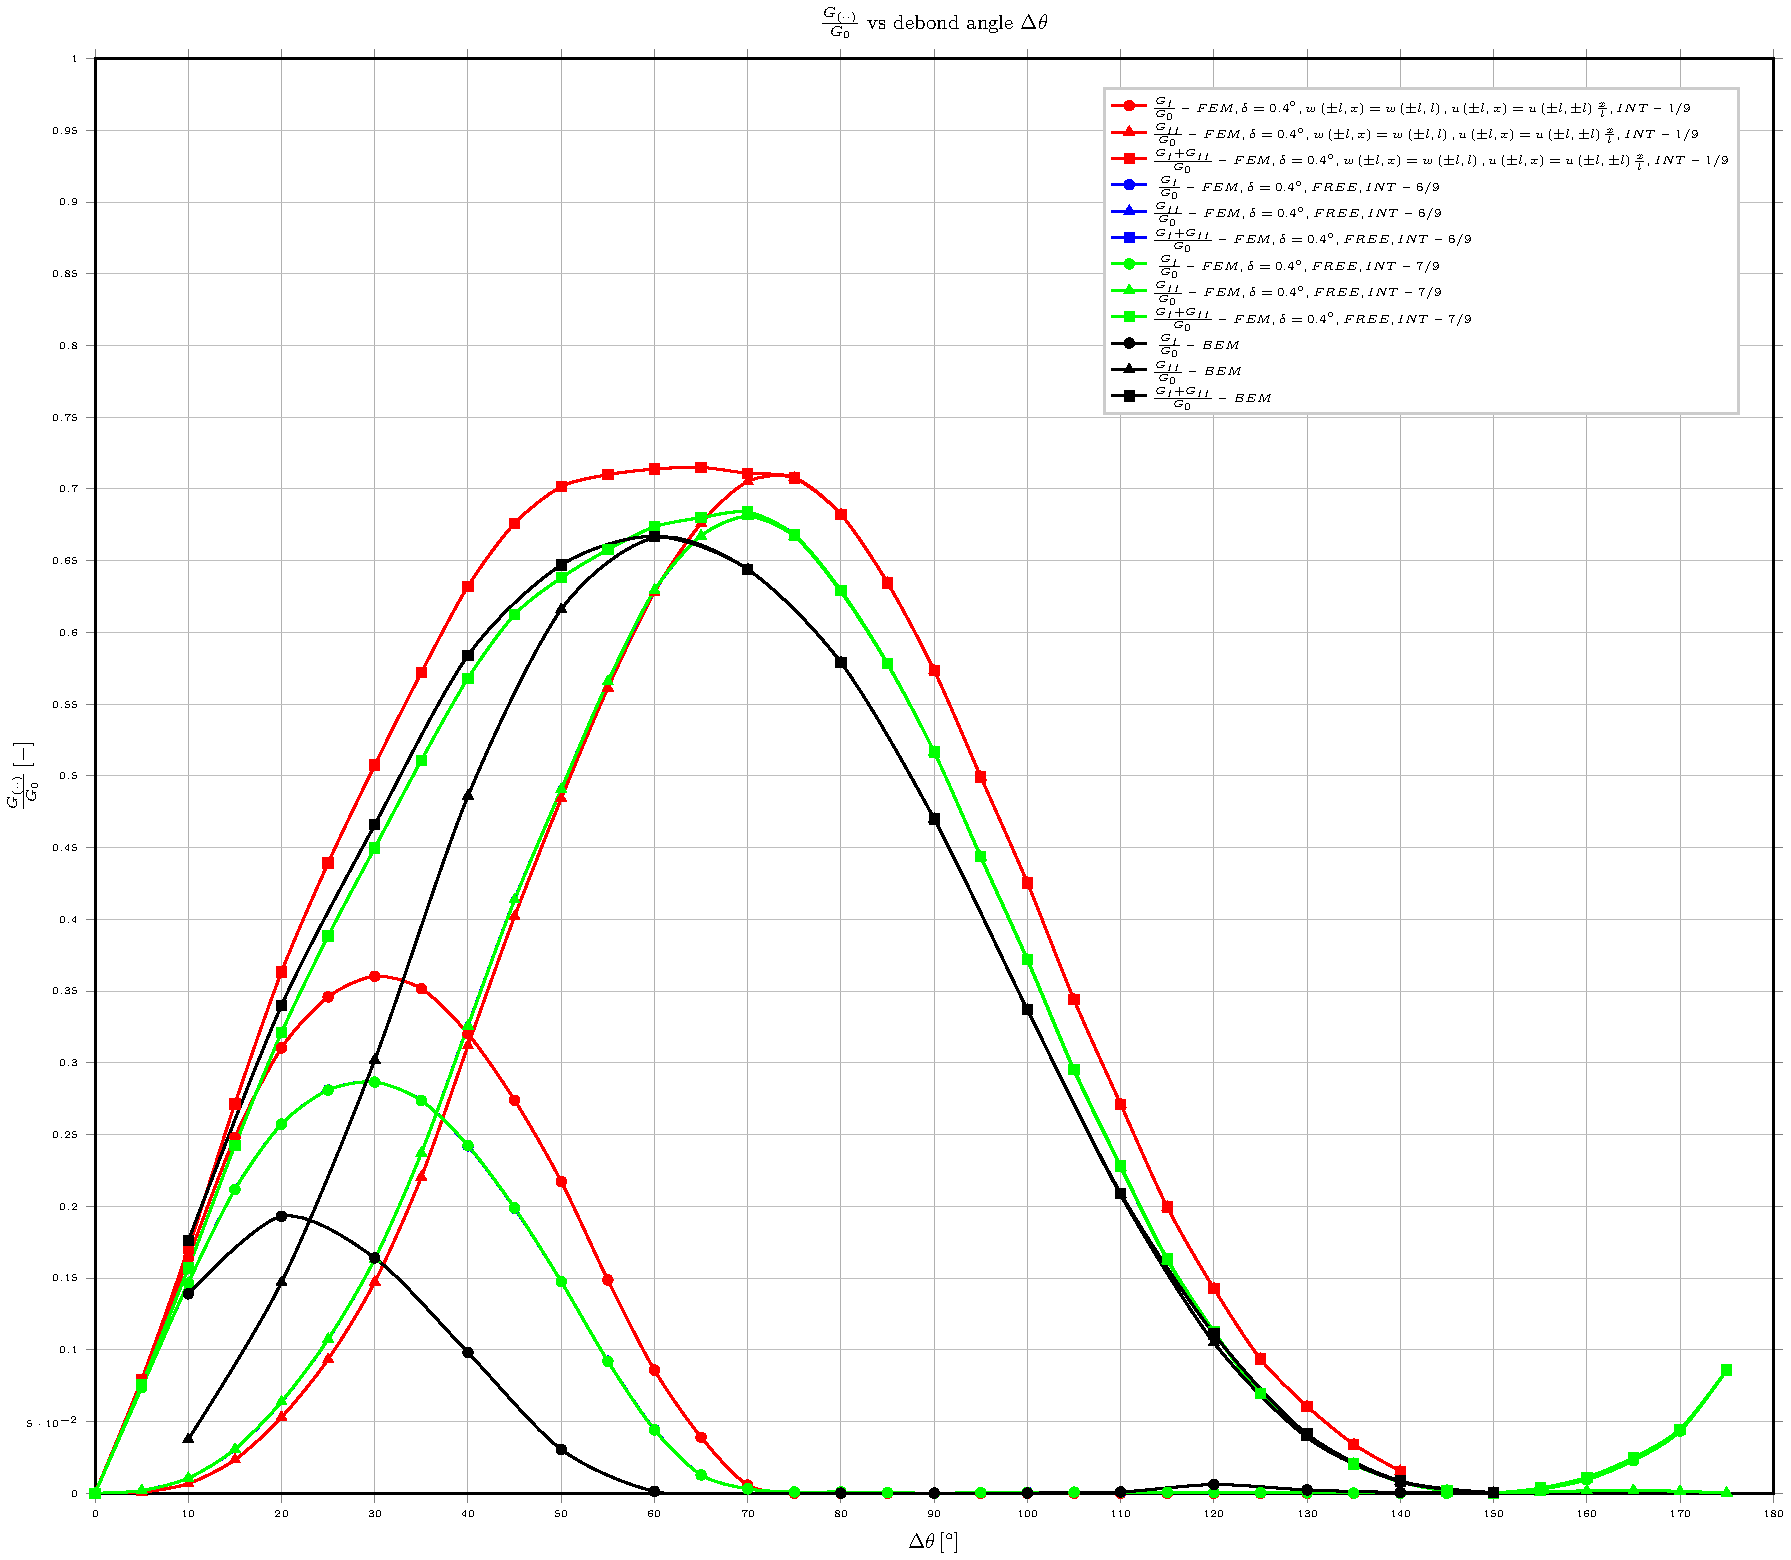
\includegraphics[height=0.7\textheight]{2017-06-01_AbqRunSummary_GsoverG0_FEM-ConnCRF-EqRF-BEM-comparison.pdf}
  \caption{\scriptsize Interface formulations 6/9 and 7/9, respectively in blue and green.}
  \label{fig:res6}
\end{figure}
\end{frame}

\begin{frame}
\frametitle{Results}
\vspace{-0.7cm}
\centering
\captionsetup[figure]{font=scriptsize,labelfont=scriptsize}
\begin{figure}[!h]
\centering
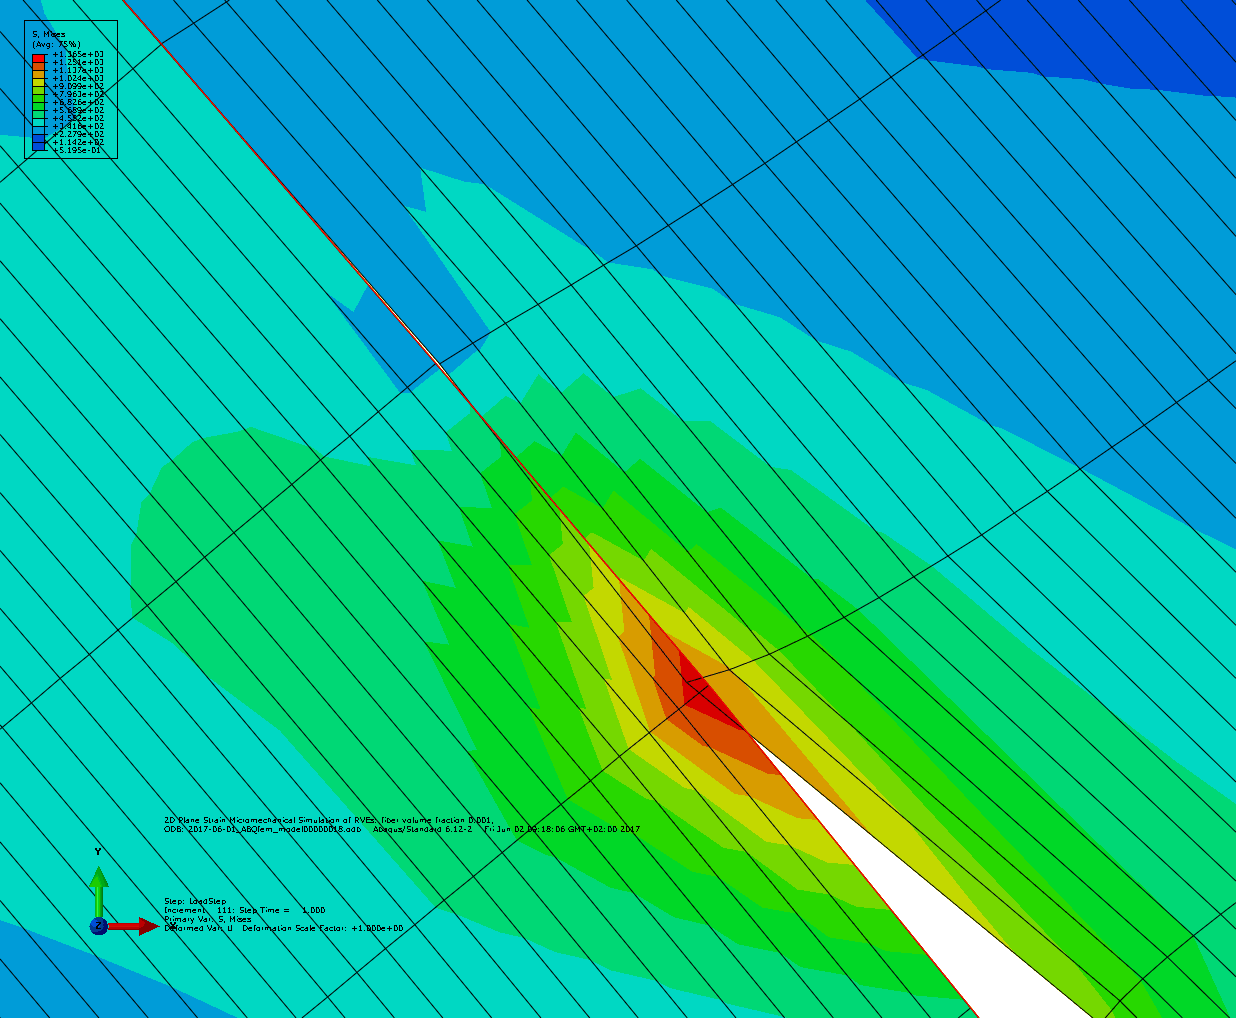
\includegraphics[height=0.7\textheight]{cracktip-detail-debondsurf.png}
  \caption{\scriptsize Crack tip in deformed configuration, surface contact pair with fracture interaction based on VCCT, $\Delta\theta=40^{\circ}$.}
  \label{fig:res6}
\end{figure}
\end{frame}

\begin{frame}
\frametitle{Results}
\vspace{-0.7cm}
\centering
\captionsetup[figure]{font=scriptsize,labelfont=scriptsize}
\begin{figure}[!h]
\centering
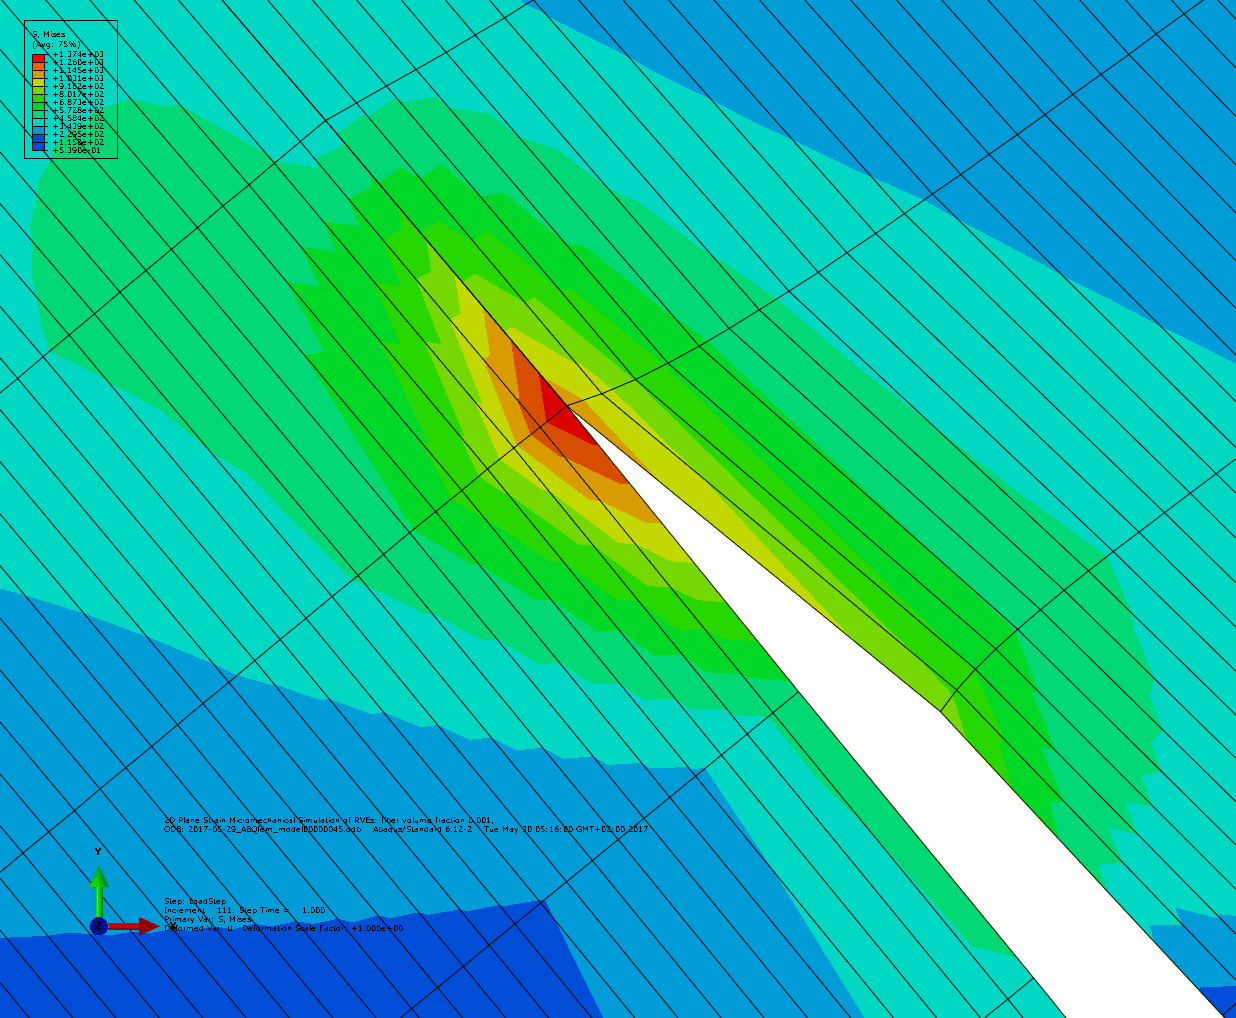
\includegraphics[height=0.7\textheight]{cracktip-detail-connel.png}
  \caption{\scriptsize Crack tip in deformed configuration, local enforcement of continuity of displacements at the interface (connector elements in the present case), $\Delta\theta=40^{\circ}$.}
  \label{fig:res6}
\end{figure}
\end{frame}

\begin{frame}
\frametitle{Results}
\vspace{-0.7cm}
\centering
\captionsetup[figure]{font=scriptsize,labelfont=scriptsize}
\begin{figure}[!h]
\centering
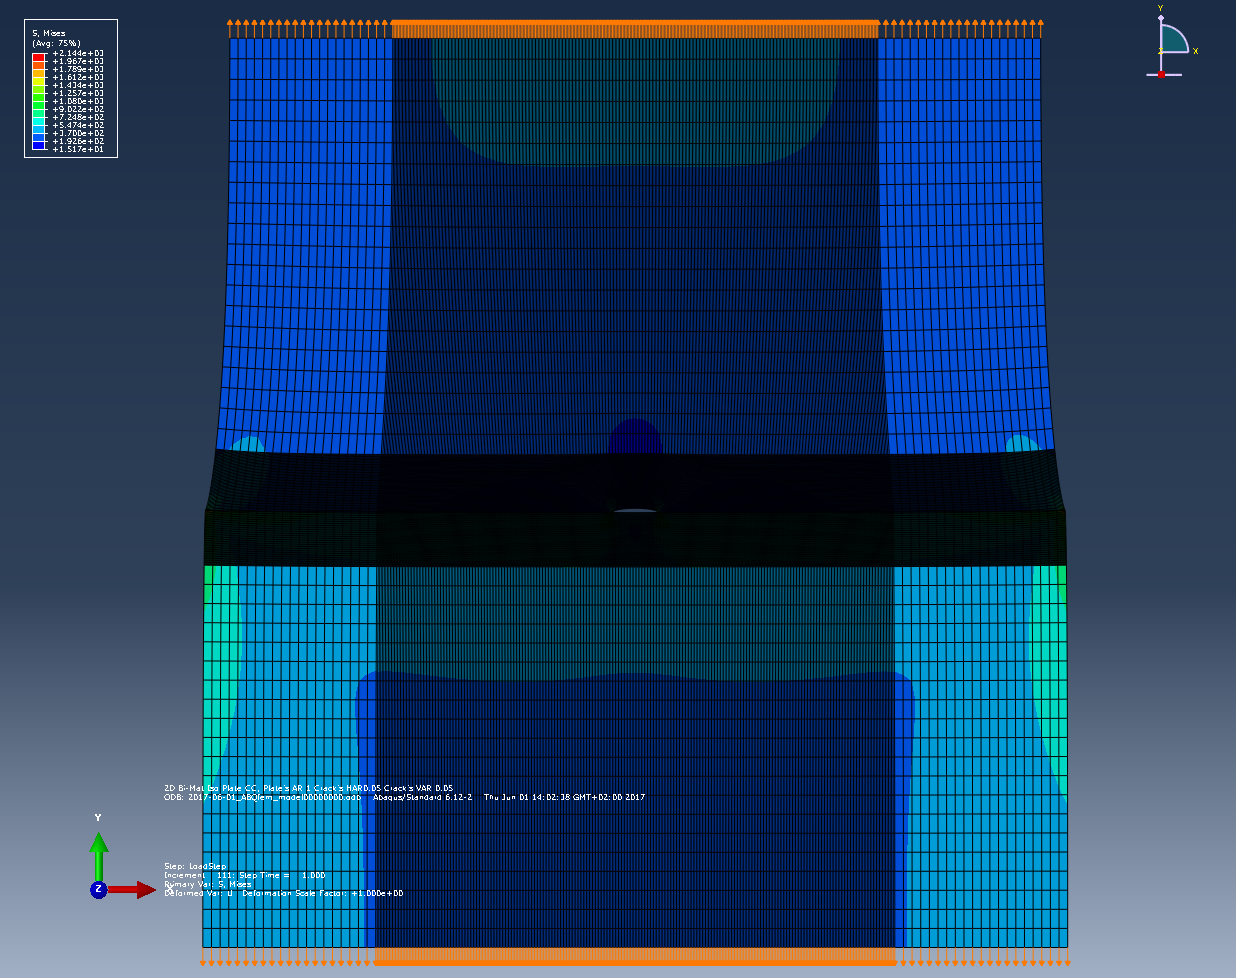
\includegraphics[height=0.7\textheight]{BIM-plate.png}
  \caption{\scriptsize FEM model of central debond between two infinite half-planes of different isotropic materials.}
  \label{fig:res7}
\end{figure}
\end{frame}






%\section{Appendices \& References}
%
%\subsection{Appendices}
%
%
%%\end{frame}
%
%\subsection{References}
%
%\begin{frame}[allowframebreaks]
%  \frametitle{References}
%    
%  \begin{thebibliography}{10}
%    
%%  \beamertemplatebookbibitems
%%  % Start with overview books.
%%
%%  \bibitem{Author1990}
%%    A.~Author.
%%    \newblock {\em Handbook of Everything}.
%%    \newblock Some Press, 1990.
% 
%    
%  \beamertemplatearticlebibitems
%  % Followed by interesting articles. Keep the list short. 
%
%\bibitem{DonaldL.Flaggs1982}
%Donald L. Flaggs, Murat H. Kural;
%\newblock {\em Experimental Determination of the In Situ Transverse Lamina Strength in Graphite/Epoxy Laminates.}
%\newblock Journal of Composite Materials, vol. 16, n. 2, 1982.
%
%\bibitem{Parvizi1978}
%Parvizi A., Bailey J.E;
%\newblock {\em On multiple transverse cracking in glass fibre epoxy cross-ply laminates.}
%\newblock Journal of Materials Science, 1978; 13:2131-2136.
%
%\bibitem{herraez2015}
%Miguel Herr\'aez, Diego Mora, Fernando Naya, Claudio S. Lopes, Carlos Gonz\'alez, Javier LLorca;
%\newblock {\em Transverse cracking of cross-ply laminates: A computational micromechanics perspective.}
%\newblock Composites Science and Technology, 2015; 110:196-204.
%
%\bibitem{Canal2012}
%Luis Pablo Canal, Carlos Gonz\'alez, Javier Segurado, Javier LLorca;
%\newblock {\em Intraply fracture of fiber-reinforced composites: Microscopic mechanisms and modeling.}
%\newblock Composites Science and Technology, 2012; 72(11):1223-1232.
%
%\bibitem{StephenW.Tsai2005}
%Stephen W. Tsai;
%\newblock {\em Thin ply composites.}
%\newblock JEC Magazine 18, 2005.
%
%
%\bibitem{ZnedekP.Bazant2002}
%Znedek P. Bazant;
%\newblock {\em Size Effect Theory and its Application to Fracture of Fiber Composites and Sandwich Plates.} 
%\newblock in Continuum Damage Mechanics of Materials and Structures, eds. O. Allix and F. Hild, 2002.
%
%
%\bibitem{RobinAmacherWayneSmithClemensDransfeldJohnBotsis2014}
%Robin Amacher, Wayne Smith, Clemens Dransfeld, John Botsis, Jo\"el Cugnoni;
%\newblock {\em Thin Ply: from Size-Effect Characterization to Real Life Design}
%\newblock CAMX 2014, 2014
%
%\bibitem{RalfCuntze}
%Ralf Cuntze;
%\newblock {\em The  World-Wide-Failure-Exercises -I  and - II for UD-materials.}
%
%
%\bibitem{Pinho}
%Pinho, S. T. and Pimenta, S.;
%\newblock {\em Size Effects on the Strength and Toughness of Fibre-Reinforced Composites.}
%
%\bibitem{PedroP.CamanhoCarlosG.DavilaSilvestreT.PinhoLorenzoIannucci2006}
%Pedro P. Camanho, Carlos G. D\'avila, Silvestre T. Pinho, Lorenzo Iannucci, Paul Robinson;
%\newblock {\em Prediction of in situ strengths and matrix cracking in composites under transverse tension and in-plane shear.}
%\newblock Composites Part A: Applied Science and Manufacturing, vol. 37, n. 2, 2006.
%
%\bibitem{P.P.CamanhoP.Maimi2007}
%P.P. Camanho, P. Maim\'i, C.G. D\'avila;
%\newblock {\em Prediction of size effects in notched laminates using continuum damage mechanics.}
%\newblock Composites Science and Technology, vol. 67, n. 13, 2007.
%
%\bibitem{Nairn1992}
%J. A. Nairn;
%\newblock {\em The Initiation and Growth of Delaminations Induced by Matrix Microcracks in Laminated Composites.}
%\newblock International Journal of Fracture, vol. 57, 1992.
%
%\bibitem{JoelCugnoniRobinAmacher2013}
%Joel Cugnoni , Robin Amacher, John Botsis;
%\newblock {\em Thin ply technology advantages. An overview of the TPT-TECA project.}
%\newblock 2014.
%
%
%  \end{thebibliography}
%\end{frame}

\begin{frame}[plain]
\frametitle{}
\end{frame}

\end{document}

